\chapter{Development of Modeling Tools for Ceramic Solid Breeders}\label{ch:modeling-development}

In this chapter we walk through the development of all the numerical tools to be used for the analysis of pebble damage in ceramic pebble beds for fusion reactors. The most important tool in the arsenal will be the pebble-scale modeling empowered by the discrete element method (DEM). The DEM code is the backbone upon which we will build two different methods of coupling to the helium purge gas; both dynamically and statically.

The core of the modeling code we employ in this dissertation come from open-sourced, crowd-supported, standard libraries. Along the process of developing the tools and adapting them to the specific needs of the ceramic breeders, I will introduce several new models and algorithms. The enhancements to the code represent a significant contribution to the design tools that will be available to solid breeder designers upon the successful completion of this dissertation.

%%%%%%%%%%%%%%%%%%%%%%%%%%%%%%%%%%%%%%%%%%%%%%%%%%%%%%%%%%%%%%%%%%%%%%%%%%%%%%%%%%%%%%%%%%%%%%
\section{Particle-scale Modeling} \label{sec:modeling-dem}

The observable, macroscopic behavior of particulate, or granular, systems is a complex function of a multitude of particle interactions. Historically, empirical relationships have been used to describe these systems as if a continuous media (see the review of \cref{sec:modeling-state}). But with the advent of the discrete element method by Cundall and Strack and the acceleration of computing power, it became practical to investigate these particulate systems at the particle scale.\cite{Cundall1979} With the discrete element method, we track all the particles in the system in a Lagrangian manner. In the ensemble, the kinematics of each particle is tracked and updated based on balances (or imbalances) of forces or energy acting upon the particle. In this section I will lie out the formulas governing interaction of particles in the DEM framework, the methods of computation, and the code used for implementation.




\section{Particle Dynamics}\label{sec:particle-dynamics}

The particles in our system are allowed translational and rotational degrees of freedom. In a packed bed, we can restrict our attention to local forces between particles; neglecting, say, non-contact forces such as van der Waals or electrostatic forces. In the first construct, we will treat the particles as if in a vacuum and leave a derivation of fluid interaction forces for \cref{sec:modeling-cfd-dem}.



%~~~~~~~~~~~~~~~~~~~~~~~~~~~~~~~~~~~~~~~~~~~~~~~~~~~~~~~~~~~~~~~~~~~~
\subsection{Particle Kinematics}

Assuming we know the contact forces acting upon particle $i$, Newton's equations of motion describe the motion of the particle. The translational and rotational for the translation degrees of freedom:

\begin{subequations}
\label{eq:newtons-second}
\begin{align}
	m_i  \ddt{\vec{r}_i}   & = m_i\vec{g} + \vec{f}_i \label{eq:newton-translational} \\
	I_i\dt{\vec{\omega}_i} & = \vec{T}_i \label{eq:newton-rotational}
\end{align}
\end{subequations}

where $m_i$ is the mass of this particle, $\vec{r}_i$ its location in space, $g$ is gravity, $I_i$ is the particle's moment of inertia, and $\vec{\omega}_i$ its angular velocity.

The net contact force, $\vec{f}_i$, represents the sum of the normal and tangential forces from the total number of contacts, $Z$, acting on this particle.

\begin{equation}
 	\vec{f}_i = \sum_{j=1}^{Z} \vec{f}_{n,ij} + \vec{f}_{t,ij}
 \end{equation} 

and the net torque, $\vec{T}_i$, is similarly,

\begin{equation}
	\vec{T}_i = -\frac{1}{2}\sum_{j=1}^{Z} \vec{r}_{ij} \times \vec{f}_{t,ij}
\end{equation}
%~~~~~~~~~~~~~~~~~~~~~~~~~~~~~~~~~~~~~~~~~~~~~~~~~~~~~~~~~~~~~~~~~~~~



%~~~~~~~~~~~~~~~~~~~~~~~~~~~~~~~~~~~~~~~~~~~~~~~~~~~~~~~~~~~~~~~~~~~~
\subsection{Linear Spring-Dashpot Model}

When Cundall and Strack first proposed the discrete element method, they used a linear spring-dashpot structure which saw the normal and tangential forces written as,

\begin{subequations}
\label{eq:dem-forces}
\begin{align}
	\vec{f}_{n,ij} &= k_{n,ij} \delta_{n,ij}\vec{n}_{ij} - \gamma_{n,ij} \vec{u}_{n,ij} 	\label{eq:normal-force} \\
	\vec{f}_{t,ij} &= k_{t,ij} \delta_{t,ij}\vec{t}_{ij} - \gamma_{t,ij} \vec{u}_{t,ij} 	\label{eq:tangential-force}
\end{align}
\end{subequations}

The fictive tangential overlap, $\delta_{t,ij}$, is truncated to so the tangential and normal forces obey Coulomb's Law, $\vec{f}_{t,ij} \le \mu_i \vec{f}_{n,ij}$ with $\mu$ as the coefficient of friction of the particle. In the first model of Cundall and Strack, the stiffness coefficients $k$ were constants and the local damping coefficients $\gamma$ were proportional to them, $\gamma \propto k$ to allow dissipation of energy and the system to reach an equilibrium. The relative normal and tangential velocities, respectively, are decomposed from the particle velocities,

\begin{subequations}
\label{eq:dem-velocities}
\begin{align}
	\vec{u}_{n,ij} &= (-(\vec{u}_i-\vec{u}_j)\cdot\vec{n}_{ij})\vec{n}_{ij} \\
	\vec{u}_{t,ij} &= (-(\vec{u}_i-\vec{u}_j)\cdot\vec{t}_{ij})\vec{t}_{ij}
\end{align}
\end{subequations}

with the unit vector $\vec{n}_{ij}$ pointing from particle $j$ to $i$

Similarly to the approach of Hertz (see \cref{sec:hertz-theory}), the surfaces of the two particles are allowed to virtually pass through each other (no deformation) resulting in normal and tangential overlaps of,

\begin{subequations}
\label{eq:dem-overlaps}
\begin{align}
	\delta_{n,ij} &= (R_i + R_j) - (\vec{r}_i -\vec{r}_j)\cdot \vec{n}_{ij} \\
	\delta_{t,ij} &= \int_{t_{c,0}}^{t} \vec{u}_{t,ij}\,\mathrm{d}\tau 
\end{align}
\end{subequations}

We have a relatively simple approach of calculating the interaction forces between particles with Eq.~\ref{eq:dem-forces} based on the kinematics of velocity and position of the interacting particles from Eq.~\ref{eq:dem-velocities} and Eq.~\ref{eq:dem-overlaps}, respectively. As the DEM evolved and drew the attention of more researchers, more complex formulas governing the forces of Eq.~\ref{eq:dem-forces} emerged. But the core approach remained the same and the models all fall into the same family of so-called `soft particle' models of DEM. A well-composed summary of the different DEM force models is given by Zhu\etal\cite{Zhu2007}.

The method used in our work is fit into the computational skeleton of Cundall and Strack's method but with non-linear spring-dashpot coefficients defined by simplified Hertz-Mindlin-Deresiewicz model; the details will be expressed in the next section.
%~~~~~~~~~~~~~~~~~~~~~~~~~~~~~~~~~~~~~~~~~~~~~~~~~~~~~~~~~~~~~~~~~~~~



%~~~~~~~~~~~~~~~~~~~~~~~~~~~~~~~~~~~~~~~~~~~~~~~~~~~~~~~~~~~~~~~~~~~~
\subsection{Hertzian Non-Linear Spring Dashpot Model}

The normal-direction (Hertz) stiffness coefficient of Eq.~\ref{eq:normal-force} is based on the Hertzian contact laws given in \cref{sec:hertz-theory}. The tangential-direction (Mindlin) stiffness coefficient follows from Brilliantov\cite{Brilliantov1996, Zhu2007, Langston1995},

\begin{subequations}
\begin{align}
	k_{n,ij} &= \frac{4}{3}E_{ij}^*\sqrt{R_{ij}^*\delta_{n,ij}} \\
	k_{t,ij} &= 8 G_{ij}^*\sqrt{R_{ij}^*\delta_{t,ij}}
\end{align}
\end{subequations}

with $G_{ij}^*$ as the pair bulk modulus,

\begin{equation}
	\frac{1}{G^*_{ij}} = \frac{2(2+\nu_i)}{E_i} + \frac{2(2+\nu_j)}{E_j}
\end{equation}

The damping coefficients, $\gamma$, arise to account for the energy dissipated from the collision of two particles\cite{DiRenzo2004, Tsuji1992, Tsuji1993}. Whether the damping coefficient is local or global and the exact form of the coefficient is more important for loosely confined granular systems and dictates the way the system approaches an equilibrium state\cite{Makse2004}. For the case of our tightly packed pebble beds, it suffices to use the efficient form of\cite{Dippel1996, Makse2004, Brilliantov1996, Zhang2005, Zhu2007},

\begin{subequations}
\begin{align}
	\gamma_n &= \sqrt{5}\beta_\text{diss}\sqrt{m^*k_{n,ij}} \\
	\gamma_t &= \sqrt{\frac{10}{3}}\beta_\text{damp}\sqrt{k_{t,ij} m^*}
\end{align}
\end{subequations}

with $\beta_\text{damp}$ as the damping ratio, and the pair mass, $\frac{1}{m^*} = \frac{1}{m_i} + \frac{1}{m_j}$. For a stable system with $\beta_\text{damp} < 1$, the damping ratio is related to the coefficient of restitution, $e$,

\begin{equation}
	\beta_\text{diss} = -\frac{\ln{e}}{\sqrt{\ln^2{e}+\pi^2}}
\end{equation}


%~~~~~~~~~~~~~~~~~~~~~~~~~~~~~~~~~~~~~~~~~~~~~~~~~~~~~~~~~~~~~~~~~~~~



%~~~~~~~~~~~~~~~~~~~~~~~~~~~~~~~~~~~~~~~~~~~~~~~~~~~~~~~~~~~~~~~~~~~~
\subsection{Time Integration}\label{sec:velocity-verlet}

Having expressed the contact mechanics of the discrete element method, we now need a means of integrating the kinematics of the particles. The most common means of marching in time with DEM is the velocity-Verlet algorithm\cite{Kruggel-Emden2008}. In this algorithm we integrate Eqs.~\ref{eq:newtons-second} with half-steps in velocity, full steps in position, and then finally the complete step in velocity (the two half-steps in velocity are often compressed into a single, full step, as we will do below). Here we will explicitly show the integration for the translational degrees of freedom. 

The force field defined by Eq.~\ref{eq:newton-translational} is rewritten in terms of the acceleration of the particle. For clarity in expression, the per-particle subscripts ($i$, $j$, etc.) will be temporarily omitted. Instead, time-varying quantities will have a subscript to refer to their temporal location. Quantities measured or evaluated at the current timestep will have subscript $t$ (note this does not refer to tangential directions!). Eq.~\ref{eq:newton-translational} is rewritten as

\begin{equation}\label{eq:newton-acceleration}
	\vec{a}_t = \vec{g} + \frac{\vec{f}_t}{m}
\end{equation}

The first step in the velocity-Verlet algorithm is to integrate the position of the particle by a full timestep based on the current timestep's velocity and acceleration. Note that the initial condition of the particle must specify both position and velocity for this step to be evaluated at the start, from then on the velocity is explicitly updated.

\begin{equation}
	\vec{r}_{t+\Delta t} = \vec{r}_t + \vec{v}_t\Delta t + \frac{1}{2}\vec{a}_t\Delta t^2
\end{equation}

The particles at new positions interact as a function of their overlaps (see Eqs.~\ref{eq:dem-forces}). Acceleration at the full timestep is then calculated from the updated forces (of Eq.~\ref{eq:newton-acceleration}). In the last computational step, the velocity at the full timestep is found from an average acceleration,

\begin{equation}
	\vec{v}_{t+\Delta t} = \vec{v}_t + \frac{\vec{a}_t + \vec{a}_{t+\Delta t}}{2}\Delta t
\end{equation}

The velocity-Verlet algorithm is an efficient means of explicitly integrating the kinematic equations for all the particles in the ensemble. The algorithm is stable with a global error of approximately $O(\Delta t^2)$ for displacement.\cite{Grubmuller1991} But, as an explicit method, the size of the timestep must be carefully chosen to avoid instabilities in the system. Stable, critical timesteps and means of circumventing unreasonably small timesteps will be addressed in \cref{sec:dem-stability}. Additionally, we have contended with the Lagrangian tracking of the particles momentum but we have still to deal with energy transfer through the packed beds which is just as important for our packed beds of ceramic breeder material. The heat transfer will be tackled in \cref{sec:dem-heat-transfer}.

In our work, we occasionally required a fully quiesced bed. To determine when this occurred, the total kinetic energy of the entire ensemble was monitored and a packed bed was considered to have completely settled once the kinetic energy of the system was less than $10^{-9}$; similar to the process described in Ref.~\cite{Silbert2002}. 
\subsection{Granular Heat Transfer}\label{sec:dem-heat-transfer}

In way analogous to that of handling the momentum of every particle in DEM with Newton's laws of motion, the Lagrangian tracking of energy of each particle is obtained via the first law of thermodynamics. We treat each particle is a single distinct object and thus do not consider any internal temperature gradients (a point which we alluded to in \cref{sec:ht-jeffreson-correction}). The temperature of particle $i$ is governed by

\begin{equation}\label{eq:thermoFirstLaw}
	m_iC_i\ddt{T_i} = Q_{s,i} + Q_{i}
\end{equation}
where $m$ and $C$ are the mass and the specific heat of the solid, respectively. Heat generation inside the particle is input with $Q_{s}$ and the total heat transferred to/from particle $i$ via conduction to all, $Z$, neighboring particles, is
\begin{equation}
	Q_i = \sum_{j=1}^Z Q_{ij}
\end{equation}

The conductive heat transfer to neighboring particles comes from inter-particle conductance formulas (derived in \cref{sec:ht-pebble-conduction}). The heat conducted between two particles is,
\begin{equation}
	Q_{ij} = H_c(T_i - T_j)
\end{equation} 
where the conductance is
\begin{equation}\label{eq:dem-conductance}
	H_c= 2k^*\left[\frac{3F_{n,ij}R^*}{4E^*}\right]^{1/3}
\end{equation}

These equations are valid for perfectly smooth spheres that obey Hertzian contact laws. The validity of this heat conductance model will be tested.

\subsubsection{Thermal Expansion}
The stresses predicted to act upon the solid breeder volume during operation of the fusion reactor arise from the differential rate of thermal expansion from the highly heated ceramic volume and the relatively cool structural container. Moreover, thermal settling motion is observed in pebble beds with cyclic heating.\cite{Tanigawa:2010cr, Vargas2007, Chen2009, Divoux2008} Both of those phenomena origin from effects of thermal expansion of individual particles in the ensemble. Therefore, we introduce a thermal expansion formula that updates the diameter of each particle as,

\begin{equation}
	d_{p,i} = d_{p_0,i}\left[1+\beta_i\left(T_i - T_0\right)\right]
\end{equation}
where $\beta_i$ is the thermal expansion coefficient (in units of \si{1/K}), $T_i$ is the temperature of the pebble at the current step, and $d_{0,i}$ is the initial diameter of the pebble at temperature $T_0$. The update of pebble diameter based on thermal expansion could be computed at every time step as it is not computationally expensive. All the same, I have left flexibility in the code to allow the computation at an arbitrary interval of time steps (typically every $\frac{1}{10000\Delta t}$)


\subsection{Numerical Implementation of DEM}\label{sec:dem-solver}


The primary computational tools used in this study is LAMMPS (Large-scale Atomic/Molecular Massively Parallel Simulator)\cite{Plimpton1995}; a classical molecular dynamics code. The package of code, maintained by Sandia National Labs (http://lammps.sandia.gov), has many features making it particularly attractive for our use on the simulation of pebble beds. LAMMPS is open-source and written in highly-portable C++ allowing customization of any feature used in modeling. LAMMPS runs with distributed-memory message-passing parallelism (MPI) and provides simple control (manual or automatic) of the spatial-decomposition of simulation domains for parallelizing. Perhaps most importantly, LAMMPS provides an efficient method for detecting and calculating pair-wise interaction forces; the largest consumer of run-time in the DEM algorithm\cite{Plimpton1995}. We build the code as a library so that LAMMPS can be coupled to other numerical tools; we use the scripting language of Python (Python 2.7) as an umbrella code to call LAMMPS routines with the full availability of Python libraries. 

LAMMPS by default provides a rudimentary method of modeling of granular particles (the term `granular' here differentiates the `discrete element' of molecules or atoms from larger-scale granular particles of powders or pebbles); LAMMPS has been used for studying granular material since at least 2001 when Silbert\etal\cite{Silbert2001} studied granular flow on inclined planes. However, the usefulness of LAMMPS for studying granular systems was greatly enhanced by LIGGGHTS (LAMMPS Improved for General Granular and Granular Heat Transfer Simulations), a suite of modules included on top of LAMMPS. LIGGGHTS has many academic and industrial contributors from around the world, with the code maintained as open-source by DCS Computing, GmbH.

Briefly, some notable features the LIGGGHTS code brings to the LAMMPS environment include: Hertz/Hooke pair styles with shear history, mesh import for handling wall geometry, moving meshes, stress analysis of imported meshes, a macroscopic cohesion model, a heat transfer model, and improved dynamic load balancing of particles on processors\cite{Kloss2011,Kloss2012}. Both LIGGGHTS and LAMMPS are distributed under the open-source codes under terms of the Gnu General Public License.

We will review some of the important physical models used in LAMMPS/LIGGGHTS as they relate to the important features we wish to investigate for packed beds of pebbles in fusion reactors.




% now we modify the elements of the model and show custom implementations of the DEM
% model based on our experiments and theories.
\section{Elasticity reduction factor}\label{sec:exp-reduction-factor}

We introduced Hertz theory in \S~\ref{hertzTheory}, and now we apply it to experiments for analysis of ceramic pebbles. The derivation of Hertz force can be found on page~\pageref{eq:hertzForce} but is given again here for reference.
\begin{align*}
F = \frac{4}{3}E^*\sqrt{R^*}\,\delta^{3/2}
\end{align*}
and, again, the relative Young's modulus and radius are
\begin{align*}
\frac{1}{E^*} & = \frac{1-\nu_i^2}{E_i} + \frac{1-\nu_j^2}{E_j} \\
\frac{1}{R^*} & = \frac{1}{R_i} + \frac{1}{R_j}
\end{align*}

In experiments where we press a ceramic pebble between two platens, we measure the travel, $s$, rather than the pebble overlap, so we modify Eq.~\ref{eq:hertzForce} to be represented in terms of travel ($s = 2\delta$). Furthermore, for a pebble ($R_i = R_p$) in contact with a smooth plane ($R_j \rightarrow \infty$), the relative radius is simply $R^* = R_p = d_p/2$.

The Hertz force is now expressed as
\begin{align}\label{eq:contact-force}
F& = \frac{1}{3}E^*\sqrt{d_ps^3}
\end{align}

Let's take a moment to discuss Eq.~\ref{eq:contact-force}. The Young's modulus of the test stand platen is a constant value. One might assume the Young's modulus of the ceramic is also a known, constant value. In that case, there should be only a single force response for every pebble of a given diameter. Using the material properties given in Ref.~\cite{Gierszewski1998} for \lit, we plot a set of parametric curves based on diameter. The properties used for an nickel-alloy platen and \lit are given in Table~\ref{tab:hertz-dp-study-props}. The curves are given in Fig.~\ref{fig:hertz-dp-dependence}.

\begin {table}[htp] %
\caption{Material properties used for \lit and nickel-alloy platen}
\label {tab:hertz-dp-study-props} \centering %
\begin {tabular}{ cccccc }
\toprule %
$E_\text{peb}$		&     $\nu_\text{peb}$	&	$E_\text{stand}$		&     $\nu_\text{stand}$	\\
(GPa)			&					&	(GPa)				&					\\\toprule
126				&	0.24				&	220					& 	0.27				\\\bottomrule
\end{tabular}
\end{table}

\begin{figure}[ht!]
\centering
\includegraphics[width = 0.75 \textwidth]{chapters/figures/hertz-dp-dependence}
\caption{Hertzian responses of \lit pebbles compressed between platens. The colormap shows pebble diameters in \si{m}. The diameters span an order of magnitude from $d_p = \si{0.2 mm}$ to $d_p = \si{2 mm}$.}\label{fig:hertz-dp-dependence}
\end{figure}

Figure~\ref{fig:hertz-dp-dependence} clearly shows that if a pebble of a given diameter is strictly obeying Hertz theory, there is only a single force-displacement curve it can follow. However, when experiments are performed on single pebbles we see quite different behavior for the F-s curves, see the curves of Fig.~\ref{fig:exp-curves}. 

\begin{figure}
        \centering
        \begin{subfigure}[b]{0.75\textwidth}
                \includegraphics[width=\textwidth]{chapters/figures/fzk-exp-colormap}
                \caption{\lis pebbles of approximately \si{0.5 mm} diameter.}
                \label{fig:fzk-exp-colormap}
        \end{subfigure}
         
        %add desired spacing between images, e. g. ~, \quad, \qquad, \hfill etc.
        %(or a blank line to force the subfigure onto a new line)
        \begin{subfigure}[b]{0.75\textwidth}
                \includegraphics[width=\textwidth]{chapters/figures/nfri-exp-colormap}
                \caption{\lit pebbles of approximately \si{1.5 mm} diameter.}
                \label{fig:nfri-exp-colormap}
        \end{subfigure}
        \caption{Force-displacement curves for two sets of experimental data, a batch of \lis pebbles and a batch of \lit pebbles. The colormap shows pebble diameters in \si{m}.}\label{fig:exp-curves}
\end{figure}

Figure~\ref{fig:fzk-exp-colormap} shows \lis pebbles as they are compressed between platens. Neglecting the handful of pebbles with very low force responses to high strain, there is a grouping of pebbles where there is a general trend that matches Fig.~\ref{fig:hertz-dp-dependence}. The smaller diameter pebbles, in blue colors, have lower force responses for a given strain. Larger pebble diameters, in yellow-orange, are slightly higher overall in their force response. Finally, the largest diameter pebble in dark red has the highest force response for a given diameter. However, while the trends are \textit{generally} similar to the theoretical Hertzian curves, there are noticeable spreads in responses. The responses of \lit pebbles of Fig.~\ref{fig:nfri-exp-colormap}, on the contrary, show almost no adherence to the expected diameter dependence of Hertz theory. 

The behavior of pebbles observed in Fig.~\ref{fig:exp-curves} lead us to conclude that variations in pebble diameter can not alone account for the variation in the F-s curves. The most reasonable source for is a variation is in the Young's modulus of pebbles in a batch. Such a conclusion is important for implementation of Hertz theory in DEM algorithms.

We hypothesize that variation in the apparent Young's modulus of each pebble is rooted in the production of the pebbles which yields pebbles with slightly different internal structures. The differences in internal structure then cause the pebble to behave with different stiffnesses than the value expected from measurements of sintered pellets of lithium ceramics. In fact, we consider the sintered pellet Young's modulus, $E_\text{sp}$, as the upper limit for the pebbles and that most will emerge with values less than $E_\text{sp}$. To quantify the deviation of each pebble's $E_\text{peb}$ from the sintered pellet, we introduce a $k$ factor, defined as the elasticity reduction factor:
\begin{align}
k = \frac{E_\text{peb}}{E_\text{sp}}
\end{align}
where
\[
k \in [0,1]
\]

If each pebble has a unique $k$ value, this would quantify the spread in elastic responses seen in the experiments. We find the value by assuming that the pebbles are, in fact, behaving in a Hertzian manner. This allows us to back-out a $k$ value, or in other words the unique $E_\text{peb}$ of that pebble by finding a best fit to the experimental curves. 

We take the sintered pebble value of Young's modulus for \lis to be $E_\text{sp} = \si{90 GPa}$ and the value for \lit to be $E_\text{sp}= \si{124 GPa}$. Then we iterate over all values of $k\in[0,1]$ and compare the Hertzian response to that pebbles force-displacement curve. At each iteration, the L2-norm of the difference between Hertzian and experimental curves is used as the `error'. The L2 norm, $A$ for a given array, $a$ is 
\begin{align}
||A||_F = \left[\sum_{i,j}\textrm{abs}(a_{i,j})^2\right]^{1/2}
\end{align}

This is a convenient way to compare the error at every point along the force-displacement curves. When the error is minimized, the elasticity reduction value corresponding the minimum is recorded for that pebble. The Hertzian curves (in black) for each pebble are plotted in green against the experimental curves in Fig.~\ref{fig:exp-hertz}. 




\begin{figure}
        \centering
        \begin{subfigure}[b]{0.75\textwidth}
                \includegraphics[width=\textwidth]{chapters/figures/fzk-hertz-colormap}
                \caption{\lis pebbles of approximately \si{0.5 mm} diameter.}
                \label{fig:fzk-hertz-colormap}
        \end{subfigure}
         
        %add desired spacing between images, e. g. ~, \quad, \qquad, \hfill etc.
        %(or a blank line to force the subfigure onto a new line)
        \begin{subfigure}[b]{0.75\textwidth}
                \includegraphics[width=\textwidth]{chapters/figures/nfri-hertz-colormap}
                \caption{\lit pebbles of approximately \si{1.5 mm} diameter.}
                \label{fig:nfri-hertz-colormap}
        \end{subfigure}
        \caption{Force-displacement curves for two sets of experimental data, a batch of \lis pebbles and a batch of \lit pebbles. The colormap shows pebble diameters in \si{m}.}\label{fig:exp-hertz}
\end{figure}



Many of the curves in Fig.~\ref{fig:fzk-hertz-colormap} seem to be fit well with a Hertzian curve with modified Young's modulus. The value of Young's modulus found for each pebble is plotted in Fig.~\ref{fig:fzk-E-plot}. The Young's modulus of pebble numbers 0 to 4 are the very 'soft' pebbles seen with very low forces on Fig.~\ref{fig:fzk-hertz-colormap}. The majority of pebbles behave with a Young's modulus between 30 and 70 \si{GPa}. On the upper end, a few pebbles acted very similar to their sintered pellet counterpart with approximate value of \si{90 GPa}.

\begin{figure}[ht!]
\centering
\includegraphics[width = 0.75 \textwidth]{chapters/figures/fzk-E-plot}
\caption{Distribution of modified Young's modulus for a batch of \lis pebbles. Most pebbles responded to compression with a Young's modulus well below the sintered pellet value of \si{90 GPa}.}\label{fig:fzk-E-plot}
\end{figure}

\begin{figure}[ht!]
\centering
\includegraphics[width = 0.75 \textwidth]{chapters/figures/nfri-E-plot}
\caption{Distribution of modified Young's modulus for a batch of \lit pebbles. All pebbles responded to compression with a Young's modulus well below the sintered pellet value of \si{126 GPa}.}\label{fig:nfri-E-plot}
\end{figure}


What remains is actually using these modified Young's modulus in DEM simulations to see if they more accurately reflect pebble bed macroscopic behavior. If so, it is assumed they will more accurately reflect the contact forces between pebbles in the ensemble.




\section{Study of Young's Modulus}\label{sec:dem-studies-youngs-modulus}

The fundamental assumption in the DEM formulation is that each pebble acts perfectly elastically and thereby adheres to Hertz theory for contacting spheres. With Hertz theory, one finds contact forces as a simple function of: the virtual overlap between two objects, the Young's modulus of the contacting material (and Poisson ratio), and radii of the two. In past studies, the Young's modulus of the ceramic materials  used in DEM simulations was taken from historical data, for instance lithium metatitanate from Ref.~\cite{Gierszewski1998}.

Based on observations of experimental data from single pebble crush data, in this study we propose a new method of obtaining the Young's modulus for a batch of ceramic pebbles as the historical values from literature are not always appropriate. Details of the motivation and physics are in \cref{sec:exp-reduction-factor}.
%~~~~~~~~~~~~~~~~~~~~~~~~~~~~~~~~~~~~~~~~~~~~~~~~~~~~~~~~~~~~~~~



%~~~~~~~~~~~~~~~~~~~~~~~~~~~~~~~~~~~~~~~~~~~~~~~~~~~~~~~~~~~~~~~
\subsection{Numerical experiments setup}
%In pebble bed breeder units, the stresses on the pebble regions are a result of thermal expansion of the relatively hot pebbles contained by relatively cool container walls. This process is a function of the coefficient of thermal expansion of the pebbles and their elevated temperature; the confined strain relates to a stress. 
We model our pebble beds undergoing a standard stress-controlled uni-axial compression up to 6 MPa. We will measure the macroscopic stress-strain for some parametrically varied pebble beds and compare the curves. At the moment of maximum stress, we can investigate the differences in contact forces of those pebble beds.

Our pebble ensemble is composed of \si{0.5 mm} diameter lithium orthosilicate pebbles. The pebble beds are initiated and packed in the same manner as \cref{sec:dem-studies-effective-conductivity}. There are two main bed groups. Set A: the first set of three beds (A.1-3) contain a single type of pebble with $E$ = \si{90 GPa}. Set B: the second set of four beds (B.1-4) contain ten types of pebbles with their Young's modulus assigned in a discrete, random way to satisfy the distribution seen from experimental data. For the DEM study, we fit to lithium orthosilicate pebbles where the average stiffness was $\bar{E} = 49$~GPa. The description of the two sets of pebble beds is visually represented in Fig.~\ref{fig:dem-types}. The pebble bed geometry was also the same used in the study of Ref.~\cite{VanLew2014}; two virtual walls in the x-direction located at $x_\text{lim} = \pm 20 R_p$, periodic boundaries at the limits of $y_\text{lim} = \pm 15 R_p$, and a total of 8000 pebbles packed into the volume to an approximate height of $z_\text{lim} = 20 R_p$.

Among both sets, a parametric study was done on pebble radius and coefficient of friction. The radii of pebbles in beds A.1, A.2, B.1, and B.2 were constant at $R_p$=.25 mm. The radii of pebbles in beds A.3, B.3, and B.4 followed a Gaussian distribution about $\bar{R}_p$ = 0.25 mm: $\mu_d = R_p$ and $sigma_d = R_p$. The coefficient of friction was set at $\mu = 0.2$ for beds A.1, A.3, B.1, and B.3; the coefficient of friction was $\mu = 0.3$ for beds A.2, B.2, and B.4.


\begin{figure}[t]
  \centering
  \includegraphics[width = 0.75 \textwidth]{chapters/figures/DEM-types}
  \caption{[color online] On the left, set A, a pebble bed with a single type, of $E = 120$ GPa. On the right, set B, is a pebble bed with 10, randomly distributed types; each type corresponds to a reduced, apparent Young's modulus as derived from experimental data.}\label{fig:dem-types}
\end{figure}
%~~~~~~~~~~~~~~~~~~~~~~~~~~~~~~~~~~~~~~~~~~~~~~~~~~~~~~~~~~~~~~~





%~~~~~~~~~~~~~~~~~~~~~~~~~~~~~~~~~~~~~~~~~~~~~~~~~~~~~~~~~~~~~~~
\subsection{Results}


A constant-velocity, uniaxial compression was applied to the pebble beds. A single cycle up to 6 Mpa was used on all the beds. The macroscopic measurements of stress-strain are shown for all the pebble beds in Fig.~\ref{fig:stress-strain}.

\begin{figure}[t]
  \centering
  \includegraphics[width = 0.75 \textwidth]{chapters/figures/stress-strain}
  \caption{[color online] Stress-strain responses of pebble beds with: squares, constant Young's modulus; and circles, Gaussian distribution of Young's modulus. The constant Young's modulus beds all had much firmer responses for all parametric cases studied here.}\label{fig:stress-strain}
\end{figure}

Naturally, the pebble beds with smaller Young’s modulus (with circle markers) are more compliant to external loads. The result is true regardless of the coefficient of friction or distribution of pebble radius studied here. Group B moved to an average strain of about 2.6\% at 6 MPa, by comparison the beds of Group A only had strained 1.9 \% on average to reach the same stress. Among the beds of each group, pebble beds with constant radius pebbles behaved virtually the same as similar pebble beds with a Gaussian distribution on radius. An increase in the coefficient of friction had a moderate impact on the overall stress-strain response. 


The parametric study here shows that the largest contributor to stress-strain response is the Young’s modulus. The coefficient of friction and radius distribution had comparatively insignificant influence. A pebble bed geometry more directly comparable to oedometric compression experiments should be used to allow direct comparison and validation of the numerical models.


At the point of peak stress for each bed, we use DEM results to visualize the distribution of contact forces among all pebbles in the ensemble. A plot of the probability distributions of all the beds together, Fig.~\ref{fig:all-contact-forces}, shows that the majority of the contacts in all the beds are equally small. There are a few overall trends we observe from the results however. The pebble beds with the constant Young's modulus are always higher for their comparable version with distributed Young's modulus. For pebble beds with comparable Young's modulii and radii, higher coefficients of friction generally have higher peak contact forces. Pebble beds' radius distributions have much less impact on peak contact forces than either coefficient of friction or Young’s modulus. Another method of comparing overall contact force distributions is to consider predictions on pebble cracking which assigns a strength value at random to pebbles in the bed, according to Eq.~\ref{eq:crush-predict}. At the point of maximum stress, this is done and the results are shown in Tab.~\ref{tab:num-crush-percent}.

While overall the predicted number of broken pebbles is small, we compare similar parameteric pebble beds and in each case pebble beds with modified Young’s modulus overall predict smaller percentages of broken pebbles. Pebble crushing is a major topic for the overall evaluation of the feasibility of ceramic pebble beds in fusion reactors. This study reveals that past DEM work on pebble crushing was likely over-predicting the extent of crushing if the Young's modulus used in the study was much larger than the realistic response of individual pebbles.

\begin{figure}[t]
  \centering
  \includegraphics[width = 0.75 \textwidth]{chapters/figures/all-contact-forces}
  \caption{[color online] Probability distribution of contact forces in all the pebble beds studied here. Elastic moduli value is the largest contributor to higher peak contact forces among pebbles.}\label{fig:all-contact-forces}
\end{figure}


\begin{table}[t]
\caption{Comparisons for the two styles of Young's modulii used in the study. }
\label{tab:num-crush-percent}\centering
\begin{tabular}{llS[table-format=3.2]}
\toprule
Bed label		& 		Parameters 								&	\text{Predicted crushed}			\\
				& 												&	\multicolumn{1}{r}{\text{\%}}		\\\otoprule
A.1				& 		$E$, $R_p$, $\mu = 0.2$          		&	0.3									\\\midrule
A.2				& 		$E$, $R_p$, $\mu = 0.3$     			&	1.0									\\\midrule
A.3				& 		$E$, $\bar{R}_p$, $\mu = 0.2$			&	0.9									\\\midrule
B.1				& 		$\bar{E}$, $R_p$, $\mu = 0.2$			&	0.6									\\\midrule
B.2				& 		$\bar{E}$, $R_p$, $\mu = 0.3$			&	0.8									\\\midrule
B.3				& 		$\bar{E}$, $\bar{R}_p$, $\mu = 0.2$		&	0.4									\\\midrule
B.4				& 		$\bar{E}$, $\bar{R}_p$, $\mu = 0.3$		&	0.7									\\\bottomrule
\end{tabular}
\end{table}
%~~~~~~~~~~~~~~~~~~~~~~~~~~~~~~~~~~~~~~~~~~~~~~~~~~~~~~~~~~~~~~~






%~~~~~~~~~~~~~~~~~~~~~~~~~~~~~~~~~~~~~~~~~~~~~~~~~~~~~~~~~~~~~~~
\subsection{Conclusions}
Models based on the discrete element method have received considerable attention by ceramic breeder researchers. The method is attractive as it is based on material properties and forgoes many of the assumptions necessary in empirical equations of effective properties for continuum models. Variation in production techniques for ceramic pebbles lead to changes in ceramic microstructure, as evident in the wide distribution of crush loads reported in past studies, \textit{e.g.} Refs.~\cite{Zhao2012,Mandal2012a}. By the same token, the different microstructures should naturally lead to variation in Young’s modulus. However up to now values of Young’s modulus used in numerical models are taken from values measured for large sintered pellets of ceramic materials. Based on single pebble experiments and the application of Hertz theory, a technique for introducing a modified Young’s modulus into DEM models has been proposed here. DEM simulations show the impact of modified pebble elasticity on both macroscopic measurements of stress-strain curves as well as mesoscopic measures of inter-pebble contact force – with major implications for prediction of pebble crushing in ceramic pebble beds. The models applying the elasticity reduction factor, $k$, predict more compliant pebble beds and smaller peak contact forces in beds and thus fewer crushed pebbles.
\section{Pebble Damage Modeling}\label{sec:failure-study}
% \cite{Hiramatsu1966}
% From , 
% \begin{align*}
% \sigma_{cr} = \cfrac{2.8}{\pi}\cfrac{F_{cr}}{4R^2}
% \end{align*}
Research on pebble damage has been taken up by others in the fusion community to predict the onset of pebble crushing as a function of an external pressure and the resulting changes to mechanical properties such as the stress-strain of the pebble bed.\cite{Annabattula2012a, Zhao2012, Zhao2013} Other fields of engineering have also employed DEM in studies of granular crushing with generally similar modeling approaches.\cite{Marketos2007,Pitchumani2004}


In modeling pebble damage, there are two main tasks: predicting when the grain crushes and what happens when it does. For the former, the task is to develop a model for predicting a pebble crushing event; \textit{i.e.} what load (mechanical or thermal) will cause a pebble to crack, shatter, fracture, etc. To tackle the latter is to develop a model which simulates the damage of that pebble; \textit{i.e.} a scheme to treat a cracked, shattered, or crushed pebble in the assembly as small particles, removed particles, or particles with modified material properties.

\begin{figure}[!t]
\centering
	\includegraphics[width=\singleimagewidth]{chapters/figures/markets-bolton-stress-strain-crushing.jpg}
	\caption{Stress-strain response of a pebble bed with crushed pebbles. Reproduced from Ref.~\cite{Marketos2007}}
	\label{fig:marketos-bolton-stress-strain}
\end{figure}

\begin{figure}[!t]
\centering
	\includegraphics[width=\singleimagewidth]{chapters/figures/annabattula-stress-strain-crushing.jpg}
	\caption{Stress-strain response of a pebble bed with crushed pebbles. Reproduced from Ref.~\cite{Annabattula2012a}}
	\label{fig:annabattula-stress-strain}
\end{figure}

This numerical study will focus on the `what happens' question. In work by Marketos and Bolton, they treated a crushed pebble very similar to Van Lew\etal~; when a pebble was damaged it was removed completely from the assembly.\cite{Marketos2007,VanLew2014} Marketos and Bolton study the stress-strain response of a pebble bed with a predictive crushing routine while we studied the effective thermal conductivity of a damaged pebble bed.

However, the technique of removing a pebble is limited by the fact that energy input into two systems being studied is not comparable. Because we have volumetric energy deposition in our simulations, the total energy pouring into the non-damaged system would be
\begin{equation}
	E_h = \frac{q'''_\text{nuc} V_\text{peb} N}{V_\text{bed}}
\end{equation}
where $N$ is the total number of pebbles of volume $V_\text{peb}$ that exist in the pebble bed of volume $V_\text{bed}$. After a crushing event, when we remove pebbles, the total amount of energy is
\begin{equation}
	E_h' = \frac{q'''_\text{nuc} V_\text{peb} \eta N}{V_\text{bed}}
\end{equation}
where $\eta$ is the percent of crushed pebbles. Obviously then, the ratio of the two heating rates is\begin{equation}
	\frac{E_h'}{E_h} = 1 - \eta
\end{equation}
and the energy deposited is not balanced between a virgin bed and one with crushed pebbles. We will attempt to address this issue.

\subsection{Modeling a Crushed Pebble}
In the DEM framework, we are limited to modeling elastic spheres. If we strictly wish to conserve mass between a solid pebble of radius $R_p$ and the crushed fragments of radius $R_c$, then the number of crushed fragments (spheres) per crushed pebble is
\begin{equation}
	N_c = \left(\frac{R_c}{R_p}\right)^{-3}
\end{equation}

Thus the number of fragments goes like the inverse of radius ratio to the third power and the number of crushed fragments to represent a single crushed pebble increases rapidly as the fragments shrink.


\begin {table}[htp] %
\caption{The particle crush fragments, $N_c$, necessary to replace a single crushed particle and obey conservation of mass (fragment number is rounded to nearest integer).}
\label {tab:rstar-Nc} \centering %
\begin {tabular}{ cc }
\toprule
$R_c/R_p$ 						& $N_c$  				\\\otoprule
0.2                             & 125                   \\    
0.25                            & 64                      \\  
0.3                             & 37               \\
0.35                            & 23               \\
0.4                             & 16                   \\
0.45                            & 11                \\
0.5                             & 8                         \\
0.75                            & 2                \\\bottomrule
\end{tabular}
\end{table}

The relationship between radius ratio and number of fragment particles is given in Fig.~\ref{fig:fragment-count}. Note that in the DEM simulation, it is impossible to insert fractions of a particle so the number of fragment pebbles is rounded to the nearest integer in the figure.

\begin{figure}[!t]
\centering
    \includegraphics[width=\singleimagewidth]{chapters/figures/crush-fragments/pebble-fragment-count.png}
    \caption{Number of fragment pebbles necessary to conserve mass increases rapidly as the size of the radius ratio ($\frac{R_c}{R_p}$) decreases.}
    \label{fig:fragment-count}
\end{figure}

In typical DEM simulations that can run within reasonable amounts of time on the machines available to me in this dissertation, a reasonable number of particles is around 10~000. Many more and the run times become impractical for study. To show how quickly the number of particles can quickly get out of hand in a simulation, if we begin with 6~000 pebbles and only 2\% break, with a radius ratio of $R_c/R_p = 0.2$, the number of pebbles to be added would be 15~000. The new particle fragments (less the crushed particles) plus the original would require 21~000 particles in the system. In our simulations, we often test the effects on effective thermal conductivity at particle crush amounts of to 10\%. For the pebble bed mentioned here, that would mean 81~000 particles in the system and it would be computationally forbidding. The result is that, for computational times, the larger crush fragment radii are desired, \textit{i.e.} $R_c/R_p > 0.3$.

However, aside from satisfying conservation of mass, we must physically insert the particle fragments into void space in the simulation domain. During the course of the simulation, when we choose to replace the pebble with the fragments, the only available room is the spherical void left over by the damaged pebble. Other constraint is the smallest sized sphere that will allow the given spheres at most dense packing. 

Dense packing of spheres inside a larger sphere is an interesting mathematical problem. \href{http://www.randomwalk.de/sphere/insphr/spisbest.txt}{Hugh Pfoertner} keeps a compiled list of many solutions for a number of particles; many solutions are his are from Gensane.\cite{gensane2003dense}

If we consider, for instance, that a radius ratio of $R_c/R_p = 0.3$ requires 37 particle fragments, then we can also find from Ref.~\cite{gensane2003dense} that 37 particles would have to be of radius 0.2406866 to fit into a single sphere of radius of unity. If we define the particle fragment radius as $R_c$, the original particle as $R_p$, and then radius of sphere necessary to hold the $N$ fragments as $R_N$, we can find a relationship between the volume of sphere $V_p$ and necessary volume $V_N$,
\begin{equation}
	r_1^* = \frac{R_c}{R_p}
\end{equation}
and
\begin{equation}
	r_2^* = \frac{R_c}{R_N}
\end{equation}
then 
\begin{equation}
	R_N = R_p \frac{r_1^*}{r_2^*}
\end{equation}
thus
\begin{equation}
	\frac{V_N}{V_p} = \left(\frac{r_1^*}{r_2^*}\right)^3
\end{equation}

If we choose a linearly spaced distribution of $r_1^*$ between 0 and 1, we can then find how many $N_c$ particles are necessary to conserve mass, then from the $N_c$ particles we can find from the database of sphere packing solutions the size of sphere that would be necessary to fit the $N_c$ particles. The calculations are carried out and shown in Fig.\ref{fig:volume-ratio}. The data in Ref.~\cite{gensane2003dense} does not go above 72 spheres so we are limited to radius ratios above about $r_1^* > 0.24$.

The plot shows that for particle fragments of reasonable numbers ($N_c\approx 20$), the volume necessary to fit the number of volume-conserving particles is greater than double the volume of the original sphere! 

\begin{figure}[!t]
\centering
    \includegraphics[width=\singleimagewidth]{chapters/figures/crush-fragments/fragment-volume-ratio.png}
    \caption{The volume necessary to house the particles of different radius ratios decreases toward unity as the radius ratio decreases. It is greater than 5 times the volume for large $r_1^*$.}
    \label{fig:volume-ratio}
\end{figure}

Therefore from the point of view of having the physical space to insert the fragments, smaller sized fragments is ideal. To insert the few number of large particles would require disrupting the packing in the region of the damaged particle.



\begin{figure}[!ht]
	\centering
	\begin{subfigure}[b]{\doubleimagewidth}
		\centering
		\includegraphics[width=\textwidth]{chapters/figures/crush-fragments/0.20-1.png}
		\caption{initial}
	\end{subfigure}
	\begin{subfigure}[b]{\doubleimagewidth}
		\centering
		\includegraphics[width=\textwidth]{chapters/figures/crush-fragments/0.20-2.png}
		\caption{final}
	\end{subfigure}
	\caption{$N_c = 8594$, $N_\text{tot} = 15430$, $R^* = 0.20$. Side view of the packing arrangement and settling for different crush fragment sizes. The small crush fragments migrate far through the height of the bed. The yellow particles are the original pebbles and the blue are fragments inserted into the system after pebble crushing.}
\label{fig:crush-settling-pictures-1}
\end{figure}
\begin{figure}[!ht]
	\begin{subfigure}[b]{\doubleimagewidth}
		\centering
		\includegraphics[width=\textwidth]{chapters/figures/crush-fragments/0.25-1.png}
		\caption{initial}
	\end{subfigure}
	\begin{subfigure}[b]{\doubleimagewidth}
		\centering
		\includegraphics[width=\textwidth]{chapters/figures/crush-fragments/0.25-2.png}
		\caption{final}
	\end{subfigure}
	\caption{$N_c = 4400$, $N_\text{tot} = 11222$, $R^* = 0.25$. Side view of the packing arrangement and settling for different crush fragment sizes. The small crush fragments migrate far through the height of the bed. The yellow particles are the original pebbles and the blue are fragments inserted into the system after pebble crushing.}
\label{fig:crush-settling-pictures-2}
\end{figure}

\begin{figure}[!ht]
	\centering
	\begin{subfigure}[b]{\doubleimagewidth}
		\centering
		\includegraphics[width=\textwidth]{chapters/figures/crush-fragments/0.35-1.png}
		\caption{initial}
	\end{subfigure}
	\begin{subfigure}[b]{\doubleimagewidth}
		\centering
		\includegraphics[width=\textwidth]{chapters/figures/crush-fragments/0.35-2.png}
		\caption{final}
	\end{subfigure}
	\caption{$N_c = 1603$, $N_\text{tot} = 8393$, $R^* = 0.35$. Side view of the packing arrangement and settling for different crush fragment sizes. The bigger fragments remain largely in place. The yellow particles are the original pebbles and the blue are fragments inserted into the system after pebble crushing.}
\label{fig:crush-settling-pictures-3}
\end{figure}
\begin{figure}[!ht]
	\begin{subfigure}[b]{\doubleimagewidth}
		\centering
		\includegraphics[width=\textwidth]{chapters/figures/crush-fragments/0.50-1.png}
		\caption{initial}
	\end{subfigure}
	\begin{subfigure}[b]{\doubleimagewidth}
		\centering
		\includegraphics[width=\textwidth]{chapters/figures/crush-fragments/0.50-2.png}
		\caption{final}
	\end{subfigure}
	\caption{$N_c = 550$, $N_\text{tot} = 7358$, $R^* = 0.50$. Side view of the packing arrangement and settling for different crush fragment sizes. The bigger fragments remain largely in place. The yellow particles are the original pebbles and the blue are fragments inserted into the system after pebble crushing.}
\label{fig:crush-settling-pictures-4}
\end{figure}
\FloatBarrier

Lastly, in this packing study we look at the displacement of the particle fragments after insertion into the system and as they come to rest in a steady state. In the images of Figs.~\ref{fig:crush-settling-pictures-1},~\ref{fig:crush-settling-pictures-2},~\ref{fig:crush-settling-pictures-3}, and~\ref{fig:crush-settling-pictures-4}, we see the initial packing of new particle fragments (in blue) settle into the interstitial gaps of the packing structure of original pebbles (yellow).

\begin{figure}[!t]
\centering
    \includegraphics[width=\singleimagewidth]{chapters/figures/crush-fragments/displacement-scatter-radius-ratios.png}
    \caption{After the particle fragments are inserted into the system they re-settle due to gravity and inter-particle forces. The small fragments travel much further throughout the bed than the large fragments.}
    \label{fig:displacement-scatter}
\end{figure}

The settling of crushing fragments is also visualized in Fig.~\ref{fig:displacement-scatter}. In this figure, the magnitude of displacement for all the crushed fragments is recorded based on the change between initial insertion location and final resting place. The displacement of the fragments is normalized against the height of the pebble bed, $H$. The fragments with $r_1^* = 0.2$ are seen to travel, on average, 10\% of the height of the pebble bed before coming to rest; some of them travel more than the entire height of the bed! In contrast, the particle fragments of size $r_1^* = 0.35$ and $r_1^* = 0.5$ travel only about 1\% of the height of the bed before coming to rest. 

The impression arises that the large displacement magnitudes of the small crush fragments would result in an overall less-dense bed with large increase in packing fraction near the floor where pebbles settle. In Fig.~\ref{fig:fragment-packing-fraction}, the packing fraction of the four different pebble beds is given. 

\begin{figure}[!t]
\centering
    \includegraphics[width=\singleimagewidth]{chapters/figures/crush-fragments/packing-fraction-height.png}
    \caption{For only 1\% of crushed pebbles, the re-settling of small pebble fragments has a small effect on the overall packing fraction of the pebble bed. In the inset, the main influence is seen in the slight increase of packing fraction within the first pebble radius of the floor.}
    \label{fig:fragment-packing-fraction}
\end{figure}


\section{Summary of DEM Modeling Development}
[this is incomplete!!]
The DEM formulation of a pebble bed allows interrogation of the micromechanical interactions that lead to macroscopic, effective properties measurable in the lab. A modified Young's modulus (fit to a probabilistic distribution) is shown to be necessary to capture the observed behavior of ceramic pebbles. The modified Young's Modulus is realized in DEM simulations with a numeric random generator satisfying a Fisher-Snedecor distribution fit to the experimental data of the pebble batch. A crush prediction algorithm was developed and implemented into DEM with a numeric random generator satisfying a Weibull distribution which assigns a critical bed-force value to each pebble. The value is constantly compared to all the contact forces acting upon a pebble in the ensemble to check for crush events. In the case of a crushed pebble, a volume-conserving pebble fragmentation script is used to simulate a broken pebble.

DEM, alone, neglects the thermal transport between pebbles and interstitial gas. Theoretically- and experimentally-based  correlations have been proposed to include stagnant gas heat transfer in DEM framework. We must address the helium influence on heat transfer within the pebble bed � two schemes are developed here








%%%%%%%%%%%%%%%%%%%%%%%%%%%%%%%%%%%%%%%%%%%%%%%%%%%%%%%%%%%%%%%%%%%%%%%%%%%%%%%%%%%%%%%%%%%%%%
\section{Dynamic Coupling of Fluid-particle, Volume-averaged Modeling} \label{sec:modeling-cfd-dem}

As we saw in Fig.~\ref{fig:keff-pressure}, even when stagnant in a bed of ceramic pebbles, helium plays a large role in the overall energy transport. A more comprehensive model of the thermophysics of a packed bed would therefore be sorely incomplete without including the contribution of helium. The first modeling approach adopted treats the helium as a volume-averaged thermofluid. Note, for shorthand I will frequently refer to the volume-averaged approach simply as the computational fluid dynamics (CFD) method, this will be sufficient to distinguish the approach from the second one introduced later. This will be the first of two approaches taken to consider the influence of helium's flow on thermal transport through the packed bed. In this approach, the fluid is considered in an Eulerian, continuum sense and the pebbles remain in the discrete, Lagrangian realm. The interactions of the fluid and solid are characterized by effective relationships in each discretized cell of fluid. The technique of coupling CFD to DEM was first proposed by Tsuji\etal.\cite{Tsuji1992} in 1992. Since that time, the CFD-DEM coupling approach has grown as a tool for granular flow research. A comparison of model formulation for CFD-DEM is discussed extensively by Zhou\etal\cite{Zhou2010}.

\section{Numerical Methodology}
% From TOFE 2014
Researchers of ceramic pebble beds for fusion reactors are concerned with damage to individual pebbles in the solid breeder volume; the accumulation of damage (\textit{e.g.} sintering, crushing) to many pebbles will ultimately have global effects on the tritium performance of the pebble bed volume.  The discrete element method provides us with the ability to probe particle-scale interactions so that we might understand, predict, and more importantly, avoid pebble damage and the morphological changes to the pebble bed associated with it. However, simulations with the DEM alone are only telling half of the story of the solid breeder. DEM models (as we are implementing them) are not able to capture the effects, neither on momentum nor energy, of an interstitial fluid. Therefore we present a modeling technique to supplement the DEM computations with a volume-averaged thermofluid model of helium (we will frequently refer to the thermofluid model as the computational fluid dynamics (CFD) method). The technique of coupling CFD to DEM was first proposed by Tsuji\etal.\cite{Tsuji1992} in 1992. Since that time, the CFD-DEM coupling approach has grown as a tool for granular flow research. A comparison of model formulation for CFD-DEM is discussed clearly by Zhou\etal\cite{Zhou2010}.

\subsection{Helium in the DEM Framework}\label{sec:cfdem-heat-transfer}

The numerical framework behind the discrete element was given in \cref{sec:particle-dynamics}. In the DEM model, each pebble obeys Newton's equations of motion. As the fluid passes through the packed bed of pebbles, it imparts a force on each individual pebble which cumulatively total to the pressure drop across the bed. To include the influence of helium, we simply augment the the linear momentum of Eq.~\ref{eq:newton-translational} to include the drag force of the fluid on the particle. The momentum balance of our Lagrangian-tracked pebble now reads,
\begin{equation}\label{eq:cfdem-dem-momentum}
	m_i  \ddt{\vec{r}_i} = m_i\vec{g} + \vec{f}_i + \beta_i V_i \Delta u_{if}
\end{equation}
where all but the last term is identical to Eq.~\ref{eq:newton-translational} but the last term accounts for the fluid. $\Delta u_{if} = u_f - u_i$, is the relative velocity between the fluid and pebble, $i$, and the inter-phase momentum exchange coefficient, $\beta_i$, acts upon the entire pebble volume, $V_i$. 

Similarly, as the helium of temperature $T_f$ passes over the particle at temperature $T_i$, energy will be exchanged. For consistency with the momentum equation, we introduce an inter-phase energy exchange coefficient (a renaming of the heat transfer coefficient) which we assume to be constant for the entire surface of the particle. The energy balance of the particle was given in Eq.~\ref{eq:thermoFirstLaw}. After adding the inter-phase energy exchange coefficient, it now reads,
\begin{equation}\label{eq:cfdem-dem-energy}
	m_iC_i \ddt{T_i} = Q_{s,i} + \sum_{j=1}^Z Q_{ij} + \beta_{E,i} A_i \Delta T_{if}
\end{equation}
where again we have only needed to add the last term to account for the energy deposited/removed by the fluid. $\Delta T_{if} = T_f - T_i$, and the inter-phase energy exchange coefficient, $\beta_{E,i}$, acts upon the pebble surface area, $A_i$.

These simple additions to the governing equations of momentum and energy of each particle are all that are necessary to introduce helium into the DEM computations. The difficulty arises in the computation of the inter-phase exchange coefficients, $\beta_i$ and $\beta_{E,i}$. We will discuss their calculations next.

\subsection{Inter-phase Exchange Coefficients}
In \cref{sec:modeling-pressure-drop}, we showed a number of correlations that engineers use to calculate the pressure drop in packed beds of spheres. The purge gas in ceramic breeders is meant to travel at very low flow rates to maximize the absorption of tritium. Furthermore, the pebble beds will always be near the close-packed limit. As such, the particle Reynolds number for these flows is often near unity and the Kozeny-Carman equation as applicable for Stokes flow is quite sufficient (see the assumptions leading to Eq.~\ref{eq:K-C-non-dim}). However, the Koch-Hill-Ladd correlation of Eq.~\ref{eq:khl-correlation} which includes terms for both the Stokes flow correlation (as a function of $\phi$) in the zero-Reynolds number limit and the viscous effects with a Reynolds number-dependent term is a general correlation that reduces to the Kozeny-Carman correlation in the close-packed, zero-Reynolds number limits. Thus for our model, we implement the KHL correlation.

The inter-phase momentum exchange coefficient is simply a re-writing of the non-dimensional drag force from Eq.~\ref{eq:khl-correlation}. The common form by Gidaspow\cite{gidaspow1994multiphase} differs from what we use here by a factor of $1-\phi$ due to definitions of the drag force. We use the form from Koch, Hill, \& Ladd.\cite{Hoef2005,Benyahia2006}
\begin{equation}\label{eq:interphase-momentum}
	\beta_{i} = \frac{18\mu_f}{d_{p,i}^2}(1-\phi_k)\phi_k F
\end{equation}
where $\mu_f$ is the fluid viscosity and the diameter of pebble $i$ is $d_{p,i}$. The packing fraction, $\phi_k$, in this equation is the local packing fraction in the fluid cell $k$. This value will differ from the global/bulk value in near-wall regions. Container walls have long been known to theoretically and experimentally force order to the packing regardless of shape of packing.\cite{Hunt1990,Benenati1962,Baird1958} For example, the void fraction ($\epsilon = 1-\phi$) in narrow annular containers using the correlation from Mueller, as a function of wall-distance in a cylinder is,\cite{Mueller1999}
\[
\epsilon = \epsilon_0 + (1-\epsilon_0)J_0(ar^*)e^{-br^*}
\]
where $r^*$ is the non-dimensional distance from the wall; here it is defined in terms of the pebble diameter, $r^* = r/d_p$. The constants, a and b, are defined in terms of the size parameter $\alpha = D/d_p$ where $D$ is the diameter of the annular tube. First, $a$ is
\[
    a= 
\begin{cases}
    7.383 - \cfrac{2.932}{\alpha - 9.864}, & \text{if }~ \alpha \geq 13\\
    8.243 - \cfrac{12.98}{\alpha + 3.156}, & \text{if} ~13 \geq \alpha \geq 2.61
\end{cases}
\]
then
\[
b = 0.304 - \cfrac{0.724}{\alpha}
\]
The bulk void fraction is found from the correlation:
\[
\epsilon_0 = 0.379 + \cfrac{0.078}{\alpha - 1.8}
\]

We then plot the packing fraction as a function of distance from the container wall for two example sizes, diameters of 20$d_p$ and 5$d_p$, in Fig.~\ref{fig:packingDist}. This example is meant to demonstrate the varying packing fraction in a packed bed that is described with a bulk or global packing fraction. The size of the discretized cell relative to the pebble will dictate how much of the void fraction variation is captured in the volume-averaged equations.

\begin{figure}[htbp]
\begin{center}
	\includegraphics[width = \singleimagewidth]{chapters/figures/annular-packing-fraction.png}
	\caption{Showing the packing fraction approach the bulk value after a few pebble diameters when the pipe is 20$d_p$ and that when the pipe is only 5$d_p$, the packing fraction at any radius is not the same as the bed average.}
	\label{fig:packingDist}
\end{center}
\end{figure}
\FloatBarrier


The inter-phase energy transfer coefficient is of the same form as a traditional heat transfer coefficient and is likewise calculated from the Nusselt number for the helium flow.
\begin{equation}\label{eq:interphase-energy}
	\beta_{E,i} = \frac{\Nu k_f}{d_{p,i}}
\end{equation}
where $k_f$ is the thermal conductivity of the fluid. Several correlations for determining the Nusselt number were given in \cref{sec:particle-convection}. We opt for the correlation provided by Li \& Mason.\cite{Li2000} Which is applicable to a wide range of Reynolds number flows [and packing fractions?].

From Eqs.~\ref{eq:interphase-momentum} and~\ref{eq:interphase-energy}, we have a formulation wherein knowledge of the flow field around our pebbles will allow calculation of dimensionless drag, $F$, and Nusselt number, $\Nu$, and the flow is coupled to our DEM computations with simple additions to the equations of motion and energy of the pebble. We next 




\subsection{Volume-averaged Thermofluid Flow}

The gas phase flow field will be treated with volume-averaging theory (VAT).\cite{Sbutega2013,whitaker1999method,Tsuji1992} The VAT allows treatment of complex porous flows with smooth continuous equations. In the VAT, we average over a discrete space to replace complex geometry with a fictitious, smooth, continuous medium in which quantities of interested are defined independently of whether specific locations in that space are, for instance, solid or gas.

In this formulation of the gas flow, we discretize the gas space with cells that are much larger than the individual particles; in the application of our CFD-DEM coupling, this meant approximately 5~6 particles per cell. With VAT, the particles themselves are not resolved in the fluid space but are simply introduced via closure terms.\cite{Sbutega2013,Horvat2006} Derivation of the governing equations of VAT can be found in Sbutega \& Catton\cite{Sbutega2013}. The momentum and energy of a fluid flow through a solid phase with volume-averaged Navier-Stokes and energy equations are applied to each cell, $k$, in the discretized fluid space,
\begin{subequations}
\begin{align}
\pder[\epsilon_k \rho_f]{t} + \nabla\cdot(\epsilon_k u_f \rho_f) &= 0\\
\pder[\epsilon_k u_f]{t} + \nabla\cdot(\epsilon_k u_f u_f) &= -\frac{\epsilon_k}{\rho_f}\nabla P_f + \nabla\cdot\left(\nu_f\epsilon_k\nabla u_f\right) - \frac{S_k}{\rho_f}\\
\pder[\epsilon_k T_f]{t} + \nabla\cdot(\epsilon_k u_f T_f) &= \nabla\left(\epsilon_k\epsilon\nabla T_f\right)-\frac{E_k}{\rho_fC_f}
\end{align}
\end{subequations}

The packing fraction in any fluid cell is calculated by summing through all the volumes of $k$ particles located in that cell
\begin{equation}
	\phi_k = \sum_{i=1}^k \frac{V_{p,i}}{\Delta V_k}
\end{equation}
where the fluid void fraction is the complement of the solid packing fraction, $\epsilon = 1 - \phi$. 

Coupling the fluid phase to the particles happens with the sink terms in momentum and energy of $S_k$ and $E_k$, respectively. They are volume-weighted sums of the drag forces and energy exchanges, respectively, for all particles in the discretized fluid cell,
\begin{subequations}
\begin{align}
	S_k &= \frac{1}{V_k}\sum_{\forall i \in k} \beta_i V_i \Delta u_{if}\\
	E_k &= \frac{1}{V_k}\sum_{\forall i \in k} \beta_{E,i} A_i \Delta T_{if}
\end{align}
\end{subequations}
The inter-phase momentum and energy exchange coefficients act as the communicators between the particle information from the DEM solver and the fluid fields from CFD. Thus the motion and energy of the fluid field are intimately coupled with the particle positions and energy, but computational time is preserved by only considering volume-averaged values in the fluid domain. %The cross-communication between fluid and solid is accomplished with a coupling routine that is explained in detail in Refs. 11, 12.


\subsection{Discussion of Methodology}
Discussion of three sets of governing equations\cite{Zhou2010}
Since the introduction of the CFD-DEM coupling methodology by Tsuji\etal~in 1993 and then Hoomans\etal~in 1996, many researchers have adopted the approach when particle-scale information of granular and fluidized beds is important.\cite{Tsuji1993,Hoomans1996} Fluidized beds have many industrial applications and are most often studied with coupled CFD-DEM tools. Review papers \cite{Zhu2007} and \cite{Deen2007}
\section{Numerical Implementation of CFD-DEM}\label{sec:cfd-dem-solver}
\section{Jeffreson Correction to Lumped Capacitance Method}\label{sec:ht-jeffreson-correction}
When incorporating helium into the DEM-based modeling, the lumped capacitance assumption for each particle in the ensemble is assumed. The assumption eases the computational efforts of solving for the temperature distribution inside each particle; each particle is treated as being isothermal. The accuracy of the lumped capacitance method is described by the Biot number,
\begin{equation}
     \Bi = \frac{hd_p}{k_r}
\end{equation} 
and for $\Bi \ll 1$ the lumped capacitance method accurately models the behavior of a solid interacting with a fluid. For $\Bi \approx 0.1$ (in cases with no heat generation), the error from the lumped capacitance method is only about 5\%. In solid breeder volumes, the particles are generally small, the solid conductivity low, and heat transfer coefficient generally is also low. This leads to small-to-moderate Biot numbers expected in the packed bed. In this section we will analyze the accuracy of the lumped capacitance and introduce a correction method to account for inaccuracies of the method at moderate Biot numbers.

I simplify the case of a packed bed and only consider a single sphere with volumetric heat generation submerged in- and thermally interacting with a fluid. The sphere will be of radius $R=d_p/2$, as shown in Fig.~\ref{fig:ParticleControlVolume}. The sphere will initially be at a uniform temperature of $T_i$. The fluid temperature will remain constant at $T_f$

\begin{figure}[ht]
	\centering
		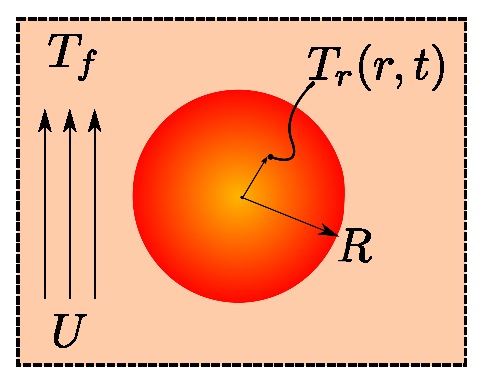
\includegraphics[width=2in]{chapters/figures/ParticleControlVolume}
	\caption[Control volume of single spherical particle in a packed bed]{Control volume of a single spherical particle in a packed bed}
	\label{fig:ParticleControlVolume}
\end{figure}


%~~~~~~~~~~~~~~~~~~~~~~~~~~~~~~~~~~~~~~~~~~~~~~~~~~~~~~~
\subsection{Lumped Capacitance Solution for Sphere}\label{sec:lumped-capacitance}
I solve for a single sphere interacting with a passing fluid, as shown in Fig.~\ref{fig:ParticleControlVolume}, while making the lumped capacitance assumption for this sphere. The solid is initially at temperature $T_0$, with constant volumetric heat generation, cooling in a fluid with constant heat transfer coefficient. The fluid will remain constant at $T_f$.

The time response of the sphere's temperature is dictated by the balance of energy to/away from the solid,  

\begin{equation}\label{eq:lc-energy-balance}
	\rho_rC_rV\frac{dT}{dt} = -hA(T-T_f) + \dot{g}V
\end{equation}

Eq.~\ref{eq:lc-energy-balance} is solved in dimensionless form with the following nondimensional parameters of temperature and time,
\begin{subequations}
\begin{align}
    \theta &= \frac{T(t) - T_f}{T_0 - T_f}\\
    \tau & = \frac{t}{R^2/\alpha}
\end{align}
\end{subequations}
where $\alpha$ is the thermal diffusivity of the sphere, $T_0$ is the initial isothermal temperature of the sphere, and $T_f$ is the constant fluid temperature. The resulting temperature distribution is,
\begin{equation}
\label{eq:theta-lc}
	\theta_{LC}=\left(1-\frac{G}{3\Bi}\right)\exp(-3\Bi \tau) + \frac{G}{3\Bi}
\end{equation}
where I have defined a dimensionless heat generation,
\begin{equation}\label{eq:nondimensional-heat-generation}
	G = \frac{\dot{g}R^2}{k(T_0 - T_f)}
\end{equation}

The energy contained in the sphere, relative to the fluid, in nondimensional terms is 
\begin{equation}
    E^*(\tau)=\frac{E(\tau)}{E_0}
\end{equation}
where $E_0$ is the initial energy of the sphere,
\begin{equation}
    E_0=\rho_rC_rV(T_0-T_f)
\end{equation}

Thus for a sphere with the lumped capacitance model, in nondimensional form, the energy is simply
\begin{equation}\label{eq:lc-energy-profile}
	E^*_{LC}(\tau) = \theta_{LC}(\tau) = \left(1-\frac{G}{3\Bi}\right)\exp(-3\Bi \tau) + \frac{G}{3\Bi}
\end{equation}

The nondimensional energy profile of Eq.~\ref{eq:lc-energy-profile} is plotted over the nondimensional time of $\tau \in [0,1/\Bi]$ in Fig.~\ref{fig:LC-sphere-in-fluid}. 

\begin{figure}[ht]
	\centering
		\includegraphics[width=\singleimagewidth]{chapters/figures/LC-sphere-in-fluid}
	\caption[Lumped Capacitance energy profile]{Lumped capacitance model: Sphere energy profile decaying from an initial value to a time of $1/\Bi$}
	\label{fig:LC-sphere-in-fluid}
\end{figure}

Reviewing Eq.~\ref{eq:theta-lc} we see that the speed of decay is dictated by the term in the exponential, $3\Bi$. Meanwhile, the steady-state value being approached is given by $\frac{G}{3\Bi} = \frac{gR}{h(T_0 - T_f)}$. It is important for this discussion to point out that because both the nondimensional heat generation and Biot number terms contain the solid conductivity, the steady-state value of the lumped capacitance model will not change for varying solid conductivity even if it leads to different Biot numbers. I will return to this point in the next section when comparing the lumped capacitance model to the exact solution when internal conduction of the solid is considered.
%~~~~~~~~~~~~~~~~~~~~~~~~~~~~~~~~~~~~~~~~~~~~~~~~~~~~~~~



%~~~~~~~~~~~~~~~~~~~~~~~~~~~~~~~~~~~~~~~~~~~~~~~~~~~~~~~
\subsection{Exact Solution for Sphere}\label{sec:analytic-sphere}

I again analyze the sphere of Fig.~\ref{fig:ParticleControlVolume} but now will account for internal temperature gradients inside the sphere. The details of the analytic solution for a sphere with heat generation interacting with a fluid is given in Appendix~\ref{sec:analytic-sphere-details}. Again, solving in terms of the nondimensional temperature and time introduced in \cref{sec:lumped-capacitance} as well as a nondimensional radius,

\begin{align*}
    \theta &= \frac{\mathbb{T}}{\mathbb{T}_0}\\
    \rho & = \frac{r}{R}\\
    \tau & = \frac{t}{R^2/\alpha}
\end{align*}

The energy conservation equation for the sphere with internal temperature gradient, in nondimensional form $\theta_{TG}$, is
\begin{equation}
    \frac{1}{\rho}\frac{\partial^2}{\partial \rho^2}(\rho\theta_{TG}) + G = \frac{\partial\theta_{TG}}{\partial \tau}
\end{equation}

With the initial condition and boundary conditions outlined in \cref{sec:analytic-sphere-details}, the nondimensional temperature distribution inside the sphere is 
\begin{equation}\label{eq:analytic-temperature-distribution}
    \theta_{TG}(\rho,\tau) = \left(\frac{G}{6} + \frac{G}{3\Bi}-\rho^2\right)  +   \sum_{n=1}^\infty \exp(-\zeta^2 \tau) \frac{\sin(\zeta_n \rho)}{\rho} \frac{Z(\zeta_n)}{N(\zeta_n)}  
\end{equation}
where $\zeta_n$ are the eigenvalues of the equation and the functions of $\zeta_n$ ($Z$,$N$,$C$) are given in \cref{sec:analytic-sphere-details}.

The accompanying nondimensional energy of the sphere is integrated to,
\begin{equation}
\label{eq:analytic-energy-profile}
    E^*_{TG}(\tau)=\left(\frac{G}{15}+\frac{G}{3\Bi}\right)+3\sum_{n=1}^\infty \exp(-\zeta^2 \tau) \frac{Z(\zeta_n)}{N(\zeta_n)} C_n(\zeta_n)
\end{equation}

I now compare the exact solution from Eq.~\ref{eq:analytic-energy-profile} to the solution of energy given by the lumped capacitance model of Eq.~\ref{eq:lc-energy-profile}. The two profiles are given in Fig.~\ref{fig:LC-analytic-sphere-in-fluid}. 

\begin{figure}[ht]
	\centering
		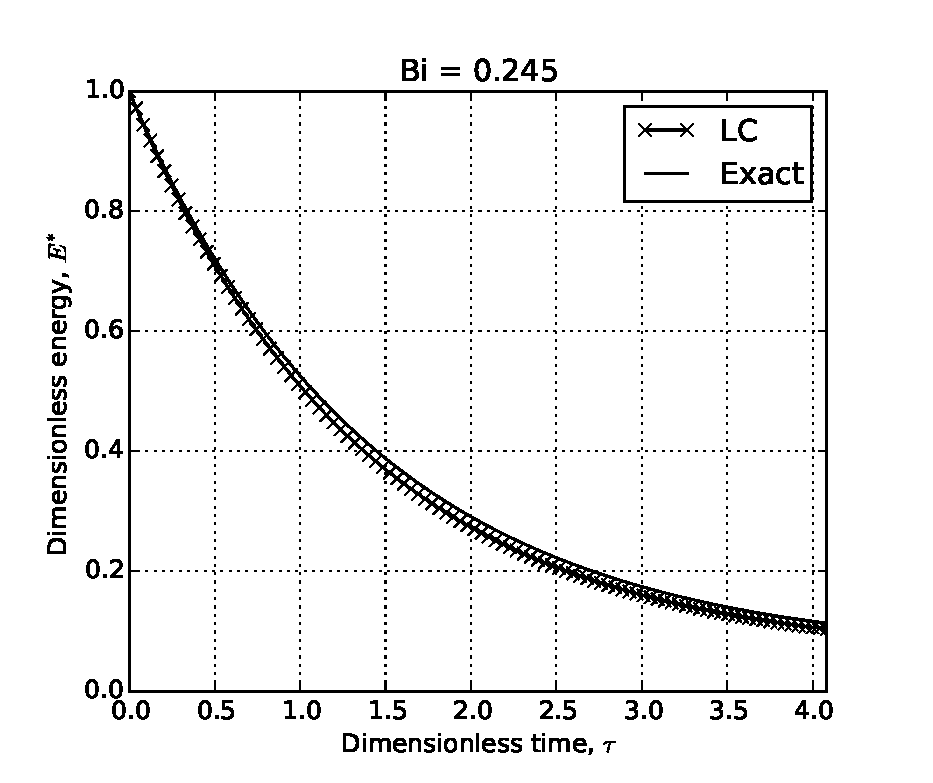
\includegraphics[width=\singleimagewidth]{chapters/figures/LC-analytic-sphere-in-fluid}
	\caption[Analytic temperature profile for $\Bi < 1$]{Analytic and lumped capacitance models: Sphere energy profile decaying from an initial value to a time of $1/\Bi$}
	\label{fig:LC-analytic-sphere-in-fluid}
\end{figure}

For the value of Biot number here, $\Bi = 0.245$, the energy profile of the analytic solution of the sphere cooling in a flow is well-captured by the lumped capacitance model. The maximum relative error over the time span, as defined by
\begin{equation}\label{eq:error}
	\text{error} = \frac{\big|E^*_{TG}(\tau) - E^*_{LC}(\tau) \big|}{E^*_{TG}(\tau)}
\end{equation}
is always less than 10\%. 

Consider now the same size sphere but with the Biot number increased by an order from: a) a conductivity of $k = k_r/10$ and b) a heat transfer coefficient of $h = 10h_f$. The two physical changes to the system result in the same Biot number ($\Bi = 2.45$) but as we can see in Fig.~\ref{fig:LC-analytic-sphere-in-fluid-Bi-2}, there are drastic differences between the energy profiles.

\begin{figure}
        \centering
        \begin{subfigure}[b]{0.5\textwidth}
                \includegraphics[width=\textwidth]{chapters/figures/LC-analytic-sphere-in-fluid-Bi-2a}
                \caption{$k \uparrow$, lumped capacitance error in the transient and steady-state.}
				\label{fig:LC-analytic-sphere-in-fluid-Bi-2a}
        \end{subfigure}%
        
          %add desired spacing between images, e. g. ~, \quad, \qquad, \hfill etc.
          %(or a blank line to force the subfigure onto a new line)
        \begin{subfigure}[b]{0.5\textwidth}
                \includegraphics[width=\textwidth]{chapters/figures/LC-analytic-sphere-in-fluid-Bi-2b}
                \caption{$h \uparrow$, lumped capacitance error mainly in the transient.}
				\label{fig:LC-analytic-sphere-in-fluid-Bi-2b}
        \end{subfigure}
        \caption[Analytic temperature profile for moderate Biot number]{Analytic and lumped capacitance models: Sphere energy profile decaying from an initial value to a time of $3/\Bi$. The same Biot number produces different results for the exact solution of a sphere with heat generation.}\label{fig:LC-analytic-sphere-in-fluid-Bi-2}
\end{figure}

Seen in Fig.~\ref{fig:LC-analytic-sphere-in-fluid-Bi-2a}, the lumped capacitance solution both over-predicts the speed at which the sphere reaches a thermal steady-state as well as the value of the steady-state. Comparatively, in Fig.~\ref{fig:LC-analytic-sphere-in-fluid-Bi-2b}, for the same Biot number, the lumped capacitance solution again over-predicts the speed to thermal steady-state by the same rate but is relatively accurate for the steady-state value itself. 

Viewing the steady-state terms of the two solutions, the source of the error becomes apparent. From Eq.~\ref{eq:analytic-energy-profile}, the steady-state term of the exact solution is
\begin{equation}
	E^*_{TG,ss}=\frac{G}{15}+\frac{G}{3\Bi}
\end{equation}

Whereas, the steady-state term of the lumped capacitance solution from Eq.~\ref{eq:lc-energy-profile} is,
\begin{equation}
	E^*_{LG,ss} = \frac{G}{3\Bi}
\end{equation}

The two steady-state values differ only by the additional term of $\frac{G}{15}$ on the exact solution. This term appears in the exact solution from integration of the temperature gradient that exists in the pebble due to volumetric heating (see \cref{sec:analytic-sphere-details}). The lumped capacitance solution assumes no internal temperature gradient in the sphere and thus by definition can not account for this $\frac{G}{15}$ term. Furthermore, the nondimensional heat generation term, $G$, given in Eq.~\ref{eq:nondimensional-heat-generation}, is importantly a function of thermal conductivity but not the heat transfer coefficient. The lack of dependence on $h$ explains the difference between steady-state values in Fig.~\ref{fig:LC-analytic-sphere-in-fluid-Bi-2}. When $\Bi$ is small, the steady state error between lumped capacitance and the exact solution is small. If only $h$ increases the error in steady-state remains small. This is demonstrated in Fig.~\ref{fig:LC-analytic-error-Bi-2b} when steady-state solutions are close. However, in Fig.~\ref{fig:LC-analytic-sphere-in-fluid-Bi-2a} as $k$ was reduced, the curves no longer converge to similar steady-states. This phenomena appears only with the combination of low conductivity materials with volumetric heating.

Even in cases without volumetric heating, when the Biot number grows large, errors appear in the transient portion of curves but ultimately converge to the same steady-state solutions. To address the inaccuracies in the time-dependent response of the lumped capacitance method with large Biot number, I make use a a correction factor such as that used by Van Lew and Xu\etal where they implemented the correction in situations without heat generation.\cite{VanLew2010,Xu2012}. In their work, they considered a heat transfer fluid interacting with a low conductivity thermal storage material. The solar thermal storage systems they analyzed often had moderate-to-large Biot numbers but they could continue to apply the lumped capacitance model in their calculations with application of a so-called Jeffreson Correction.\cite{jeffreson409} However, because their applications did not involve heat generation, I must validate its usefulness for application in our pebble beds absorbing nuclear heat.
%~~~~~~~~~~~~~~~~~~~~~~~~~~~~~~~~~~~~~~~~~~~~~~~~~~~~~~~





%~~~~~~~~~~~~~~~~~~~~~~~~~~~~~~~~~~~~~~~~~~~~~~~~~~~~~~~
\subsection{Jeffreson Correction for Sphere with Nuclear Heating}
The correlation to correct the heat transfer coefficient due to solids with large Biot number is given by Jeffreson as,\cite{jeffreson409}
\begin{equation}
	h_{p}=\frac{h}{1+\Bi/5}
\end{equation}
where $h_p$ is the modified heat transfer coefficient of the particle with an internal temperature gradient. As the Biot number increases, the modified heat transfer coefficient decreases. THe form of this correlation works to effectively slow down the rate of heat removed by the passing fluid. Recall the curves of Fig~\ref{fig:LC-analytic-sphere-in-fluid-Bi-2}. where the lumped capacitance solution over-predicted the speed with which the energy decayed towards steady-state. A modified Biot number can then also be written as
\begin{equation}\label{eq:jeffreson-correction-bip}
	\Bi_p = \frac{h_p d}{k_r} = \frac{\Bi}{1+\Bi/5}
\end{equation}

Applying the Jeffreson Correction to Eq.~\ref{eq:theta-lc}, the modified lumped capacitance solution is written now in terms of the modified Biot number,
\begin{equation}
\label{eq:theta-jc-bip}
	\theta_{JC}=\left(1-\frac{G}{3\Bi_p}\right)\exp\left(-3\Bi_p \tau\right) + \frac{G}{3\Bi_p}
\end{equation}
and thereby Eq.~\ref{eq:lc-energy-profile} also yields
\begin{equation}\label{eq:jc-energy-profile}
	E^*_{JC}(\tau) = \left(1-\frac{G}{3\Bi_p}\right)\exp\left(-3\Bi_p \tau\right) + \frac{G}{3\Bi_p}
\end{equation}

The energy profiles from the lumped capacitance model (LC), the Jeffreson correction (JC), and the exact solution are all plotted together in Fig.~\ref{fig:LC-JC-analytic-sphere-in-fluid-Bi-2}. Barely visible under the JC solution are teh curves from the exact solution. The Jeffreson correction to the lumped capacitance method allows the simple modeling approach of the lumped capacitance method to capture the proper transient as well as steady-state values for this sphere with a moderately sized Biot number. 

\begin{figure}
        \centering
        \begin{subfigure}[b]{0.5\textwidth}
                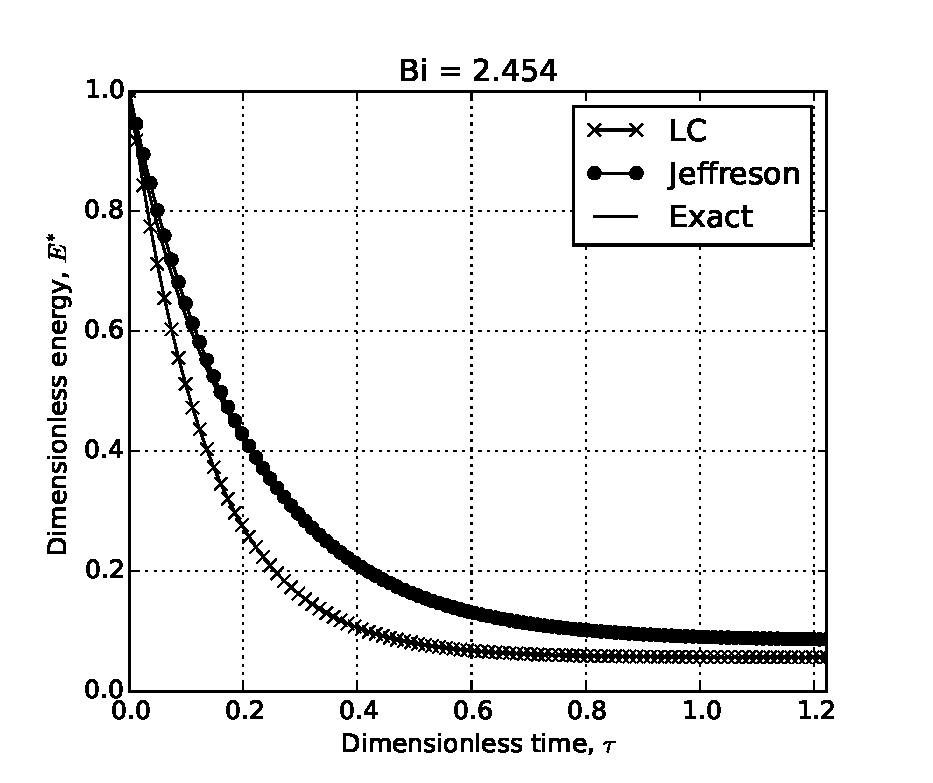
\includegraphics[width=\textwidth]{chapters/figures/LC-JC-analytic-sphere-in-fluid-Bi-2a}
                \caption{The Biot number increased from a decrease in the solid conductivity.}
				\label{fig:LC-JC-analytic-sphere-in-fluid-Bi-2a}
        \end{subfigure}%
        
          %add desired spacing between images, e. g. ~, \quad, \qquad, \hfill etc.
          %(or a blank line to force the subfigure onto a new line)
        \begin{subfigure}[b]{0.5\textwidth}
                \includegraphics[width=\textwidth]{chapters/figures/LC-JC-analytic-sphere-in-fluid-Bi-2b}
                \caption{The Biot number increased from  an increase in the heat transfer coefficient.}
				\label{fig:LC-JC-analytic-sphere-in-fluid-Bi-2b}
        \end{subfigure}
        \caption[Jeffreson correction for moderate Biot number based on conductivity]{Analytic, lumped capacitance model, and LC model with Jeffreson correction: Jeffreson correction corrects for transient and steady-state errors of lumped capacitance.}\label{fig:LC-JC-analytic-sphere-in-fluid-Bi-2}
\end{figure}

\begin{figure}
        \centering
        \begin{subfigure}[b]{0.5\textwidth}
                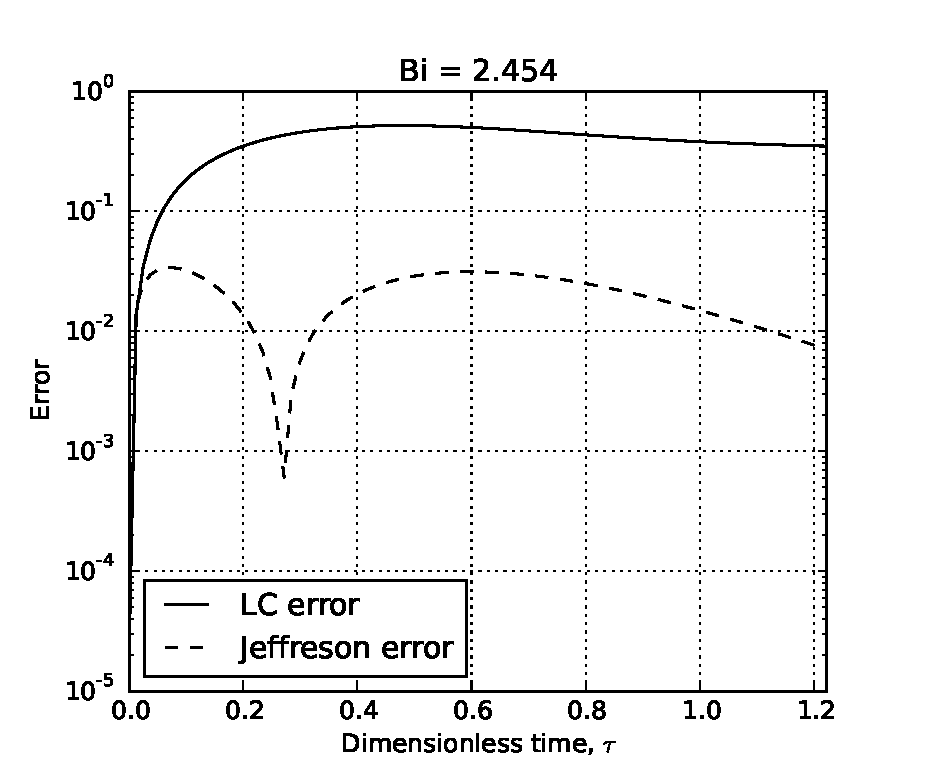
\includegraphics[width=\textwidth]{chapters/figures/LC-JC-analytic-error-Bi-2a}
                \caption{The Biot number increased from a decrease in the solid conductivity.}
				\label{fig:LC-JC-analytic-error-Bi-2a}
        \end{subfigure}%
        
          %add desired spacing between images, e. g. ~, \quad, \qquad, \hfill etc.
          %(or a blank line to force the subfigure onto a new line)
        \begin{subfigure}[b]{0.5\textwidth}
                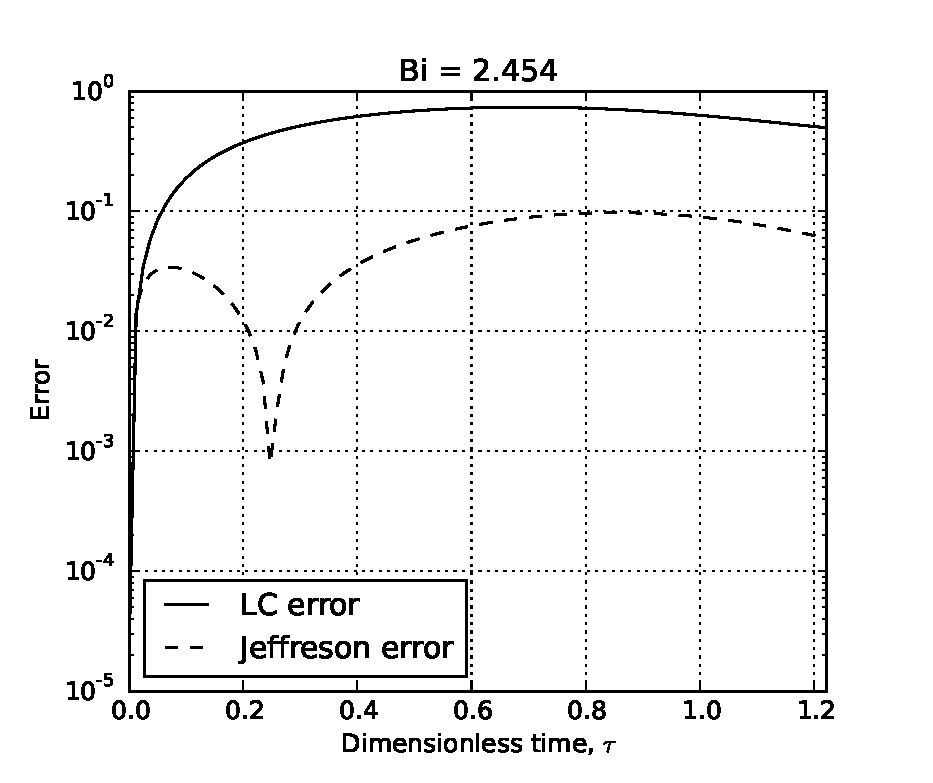
\includegraphics[width=\textwidth]{chapters/figures/LC-JC-analytic-error-Bi-2b}
                \caption{The Biot number increased from  an increase in the heat transfer coefficient.}
				\label{fig:LC-JC-analytic-error-Bi-2b}
        \end{subfigure}
        \caption[Error of lumped capacitance and Jeffreson correction for moderate Biot number]{Error of lumped capacitance and reduced error of the model with Jeffreson correction for moderate Biot number.}\label{fig:LC-JC-analytic-error-Bi-2}
\end{figure}

To look more closely, we view the instantaneous error (see Eq.~\ref{eq:error}) in Fig.~\ref{fig:LC-JC-analytic-error-Bi-2}. For the value of $\Bi > 1$ due to either low conductivity (Fig.~\ref{fig:LC-JC-analytic-error-Bi-2a}) or high heat transfer coefficient (Fig.~\ref{fig:LC-JC-analytic-error-Bi-2b}), the error in the Jeffreson correction is always under 10\%; often closer to only 1\%. This is in opposition to the standard lumped capacitance method which has 50-80\% error for both transient and steady-state values.

The lumped capacitance method allows researchers to simplify transient, conjugate heat transfer problems to a situation with an isothermal solid. In the discrete element method, the assumption of isothermal solid is innate in the framework of the method. With the implementation of the Jeffreson correction in the discrete element method, we have confidence in the fidelity of the heat transfer with the helium flow for moderately sized Biot numbers. The Jeffreson correction will be implemented into the DEM computations via Eq.~\ref{eq:jeffreson-correction-bip}. 
%~~~~~~~~~~~~~~~~~~~~~~~~~~~~~~~~~~~~~~~~~~~~~~~~~~~~~~~

\section{Summary of CFD-DEM Modeling Development}

Researchers of ceramic pebble beds for fusion reactors are concerned with damage to individual pebbles in the solid breeder volume; the accumulation of damage (\textit{e.g.} sintering, crushing) to many pebbles will ultimately have global effects on the tritium performance of the pebble bed volume.  The discrete element method provides us with the ability to probe particle-scale interactions so that we might understand, predict, and more importantly, avoid pebble damage and the morphological changes to the pebble bed associated with it. However, simulations with the DEM alone are only telling half of the story of the solid breeder. DEM models (as we are implementing them) are not able to capture the effects, neither on momentum nor energy, of an interstitial fluid. 


CFD-DEM begun as a tool to study fluidized beds
Benchmarked against common jet-spout fluidized beds with light-to-medium packing

CFD-DEM has not yet been applied to packed beds with nuclear heating such as our breeder blanket volumes
Fluid-solid heat transfer correlation was developed for non-heat-generation situations
The lumped capacitance assumption is made for the particles

We test the validity of lumped capacitance assumption when pebbles experience heat generation \& introduce a correction


Retains pebble-scale micromechanical interaction information necessary for pebble damage modeling

Computational resources conserved with volume-averaged treatment of fluid
Closure of particle-fluid heat transfer equations via experimental correlations for heat transfer coefficient on DEM particles

A modified heat transfer coefficient is derived and introduced to account for not satisfying Biot number assumption in lumped-capacitance analysis
Accounts for internal temperature gradients with negligible computational overhead

Simplicity of model sacrifices simulation of complex flow fields � unclear if this is an acceptable simplification











%%%%%%%%%%%%%%%%%%%%%%%%%%%%%%%%%%%%%%%%%%%%%%%%%%%%%%%%%%%%%%%%%%%%%%%%%%%%%%%%%%%%%%%%%%%%%%
\section{Static Coupling of Fluid-particle, Complete Modeling}\label{sec:modeling-lbm}
The volume-averaged approach of the CFD-DEM coupling is an effective and efficient method for solving transiently-coupled helium flow and pebble interaction via volume-averaging techniques for the fluid. However, there are situations when a complete knowledge of the tortuous flow of the interstitial helium is desired. Because the CFD-DEM solver does not resolve the pathways on the particle scale, knowledge of precise helium flow is not possible with that scheme. Therefore I have also investigated a method of linking our DEM pebble beds with lattice-Boltzmann solvers. 

The lattice-Boltzmann method (LBM) to fluid simulations is a growing field of numerical modeling with a rich historical development. As the LBM approach is relatively new and its governing equations seem much more esoteric than the familiar conservation equations from continuum modeling, I will first go through some of the notable evolutions of the modeling history and the background physics leading to the governing equations -- which lend themselves to relatively straightforward numerical implementation. Certainly this short study cannot do justice to a proper explanation of the underlying physics. References~\cite{Chen1998a,Viggen2009,Sukop2007,Chopard2002,succi2001lattice} should be read by those curious for an excellent and thorough description of the physics, modeling approaches, and applications of LBM theory to fluid dynamics problems.

The lattice-Boltzmann is named after its mother: lattice gas automata, and its father: the Boltzmann equation from statistical mechanics. Understandably, the lattice-Boltzmann method is meant to inherit many of the advantages from both of its parents. We begin with a brief introduction to the Boltzmann equation for the statistical behavior of non-equilibrium thermodynamic systems. Then we will introduce some of the lattice gas automata predecessors to the current lattice-Boltzmann method.

\subsection{Discretized Boltzmann Equation}\label{sec:lbm-intro}

In the realm of statistical mechanics, suppose we wish to know, at a certain time $t$, how many particles exist at a given location, $\vec{x}$, that have momentum, $\vec{p}$. We define a number,
\begin{equation}
	n = f(\vec{x},\vec{p},t)\mathrm{d}\vec{x}\mathrm{d}\vec{p}
\end{equation}
as the number of $n$ particles in the system that exist within the coordinates of $\mathrm{d}\vec{x}$ and momenta $\mathrm{d}\vec{p}$ at that instant. $f(\vec{x},\vec{p},t)$ is the probability density function representing the odds of finding a particle per phase space ($\vec{x},\vec{p}$) at a moment in time, $t$.

Now let us assume we apply a small force, $\vec{F}$, to all the $n$ particles and then increment time by $\mathrm{d}t$. Assuming further that none of the particles collide (with each other or any other particles in the system), the particles will have moved an amount $\vec{x} + \frac{\vec{p}}{m}\mathrm{d}t$. The particles will all also have had their momentum changed by an amount $\vec{p} + \vec{F}\mathrm{d}t = \vec{p} + \mathrm{d}\vec{p}$. In other words, those $n$ particles are now found in the phase space of
\begin{equation}
 	n = f(\vec{x} + \frac{\vec{p}}{m}\mathrm{d}t,\vec{p} + \mathrm{d}\vec{p},t + \mathrm{d}t)\mathrm{d}\vec{x}\mathrm{d}\vec{p}
 \end{equation}

The number of particles in the two moments of time are conserved, so we can also say
\begin{equation}
	f(\vec{x} + \frac{\vec{p}}{m}\mathrm{d}t,\vec{p} + \mathrm{d}\vec{p},t + \mathrm{d}t)\mathrm{d}\vec{x}\mathrm{d}\vec{p} = f(\vec{x},\vec{p},t)\mathrm{d}\vec{x}\mathrm{d}\vec{p}
\end{equation}

Next we relax the assumption of no collisions. If we focus our attention of the phase space as before, some of the particles that began at $(\vec{x},\vec{p},t)$ will not arrive at the phase space of $(\vec{x} + \frac{\vec{p}}{m}\mathrm{d}t,\vec{p} + \mathrm{d}\vec{p},t + \mathrm{d}t)$. By the same measure, some particles that began in some other phase space \textit{will} arrive in $(\vec{x} + \frac{\vec{p}}{m}\mathrm{d}t,\vec{p} + \mathrm{d}\vec{p},t + \mathrm{d}t)$. Now the number of particles is not conserved and we write the net number of particles having left/entered this phase space as
\begin{equation}
	\Omega\mathrm{d}\vec{x}\mathrm{d}\vec{p}\mathrm{d}t
\end{equation}
where $\Omega$ is classically referred to as the collision operator. This function dictates the evolution of particles after a collision (what phase space they leave/enter). Treatment of the collision operator is itself a source for discussion but we leave it as a generic operator. Thus the balance of particles is now
\begin{equation}\label{eq:particle-balance}
	f(\vec{x} + \frac{\vec{p}}{m}\mathrm{d}t,\vec{p} + \mathrm{d}\vec{p},t + \mathrm{d}t)\mathrm{d}\vec{x}\mathrm{d}\vec{p} - f(\vec{x},\vec{p},t)\mathrm{d}\vec{x}\mathrm{d}\vec{p} = \Omega\mathrm{d}\vec{x}\mathrm{d}\vec{p}\mathrm{d}t
\end{equation}

To be precise, to arrive at the collision operator, $\Omega$, in the form we have used in Eq.~\ref{eq:particle-balance}, it is required to make a few more assumptions on the system. Following Ludwig Boltzmann, we assume: the particles are dilute, point-like, and structureless that only interact via short-range two-body potentials. Another famous assumption from Boltzmann was of \textit{Stosszahlansatz} (molecular chaos) which allow the inter-particle interactions to be described only in terms of their local binary collisions with very long paths through free space between collisions.\cite{succi2001lattice} For the sake of this discussion, we will just accept the formulation of Eq.~\ref{eq:particle-balance} as the evolution equation for the particles in our system. 

As a side note, after taking the multi-dimensional Taylor expansion of Eq.~\ref{eq:particle-balance}, we arrive at the the recognizable Boltzmann equation,
\begin{equation}\label{eq:boltzmann-continuum}
	\left[\vec{c}\cdot\nabla + \vec{F}\cdot\partial_\vec{p}  + \partial_t\right] f(\vec{x},\vec{p},t) = \Omega
\end{equation}
where $\vec{c} = \vec{p}/m$. In the form of Eq.~\ref{eq:boltzmann-continuum}, it is clear how the Boltzmann equation describes the evolution in a continuous way. There are an infinite number of directions and momenta for the particles to evolve into/from. 

However, let us discretize onto the directions of nodes in a lattice for computability. Returning to the form of Eq.~\ref{eq:particle-balance}, we normalize the mass such that $m=1$, making $\vec{p}/m = \vec{p}=\vec{c}$. Then we only allow the continuum velocity to only point in the discrete $i$ directions of neighboring nodes, $\vec{c}\rightarrow\vec{c}_i$. In discrete increments of time, we also write the collision operator in a discrete form, $\Omega\mathrm{d}t \rightarrow \Omega_i(\vec{x},t)$. Thus, Eq.~\ref{eq:particle-balance} becomes,
\begin{equation}
	f_i(\vec{x}+\vec{c}_i\Delta t, t + \Delta t) - f_i(\vec{x},t) = \Omega_i(\vec{x},t)
\end{equation}

Lastly, if we assume that we are using time units that have been normalized such that $\Delta t = 1$, the above becomes
\begin{equation}\label{eq:boltzmann2lbe}
	f_i(\vec{x}+\vec{c}_i, t + 1) - f_i(\vec{x},t) = \Omega_i(\vec{x},t)
\end{equation}

In the form of Eq.~\ref{eq:boltzmann2lbe}, our discretized version of the Boltzmann equation for statistical mechanics will be seen to be identical to a lattice-based formulation that will be arrived at purely from the point of view of the lattice gas automaton.



\subsection{Lattice Gas Automata}

In a broad sense, lattice gas automata (LGA) simulated the behavior of individual particles with a simple boolean approach where basic collision rules were defined at nodes in a lattice. As particles approached the node from neighboring nodes at a given time, the rules would dictate the direction of the particle at the next moment in time. Computationally, the particles were simply represented with boolean operators that said either 1: a particle existed at that node in that direction; or 0: no particle existed at that node in that direction. Conceptually, the particles can be thought of as hard spheres that would collide on nodes of a lattice; collisions would send the particles rebounding along discrete directions toward neighboring nodes. The restraint on collision rules required that they obey conservation of mass and momentum. 

The earliest LGA was a two-dimensional model by Hardy, Pomeau, and de Pazzis (HPP) in 1973.\cite{Hardy1975} The HPP model applied basic conservation rules that particles had to obey at each node. From the streaming particles, macroscopic units could be extracted. For instance, the particle density at a node is found from the total number of boolean particles at that node,
\begin{equation}
	\rho(\vec{x},t) = \sum_i n_i(\vec{x},t)
\end{equation}
where $n_i(\vec{x},t)$ are the particles occupying the node at $\vec{x}$ at time $t$ with a velocity of $\vec{c}_i$. As mentioned, the value of $n$ is a boolean value of 1 or 0 if the particle is present or not. Similarly, the momentum at the node is found as,
\begin{equation}
	\rho(\vec{x},t)\vec{u}(\vec{x},t) = \sum_i \vec{c}_in_i(\vec{x},t)
\end{equation}
where $\vec{u}(\vec{x},t)$ is the mean velocity of the particles at the node at that time.

The HPP model proved promising compared to other numerical methods for a number of reasons. Importantly, the boolean nature of the automata meant that the solution was not only exact (not susceptible to any round-off errors of floating point numbers) but each node required only four bits to completely describe the state (each bit described the four directions of traveling particles in the two dimensional node).\cite{Hardy1975} Furthermore, the HPP model benefited from the inherently parallel nature of all LGA simulations. The collision behavior at any given node is independent of all other nodes; the nodes only need to communicate when particles stream to neighbors.\cite{succi2001lattice}

The LGA method was given considerable more attention after 1986 when Frish, Hasslacher, and Pomeau (FHP) showed it to be possible to solve lattice gas automata simulations that were ostensibly equivalent to Navier-Stokes equations (in two dimensions).\cite{Frisch1986} Descriptions of the hexagonal lattice used in the FHP model can be found in the textbooks of Succi (Ref.~\cite{succi2001lattice}) and Sukop \& Thorne (Ref.~\cite{Sukop2007}). The FHP method gave qualitatively beautiful reproductions of hydrodynamic phenomena.

Other such LGA models were developed with the same fundamental construction as the two models mentioned here. All the models followed the same basic form of evolution of the particles. Following the form of Ref.~\cite{chopard1998cellular},
\begin{equation}\label{eq:lattice-evolution}
	n_i(\vec{x}_i + \vec{c}_i,t+1) - n_i(\vec{x},t) = \Omega_i(\vec{x},t)
\end{equation}
where, in lattices, $\Delta t = 1$ is a standard normalization. After already deriving the Boltzmann equation, Eq.~\ref{eq:lattice-evolution} is quite familiar. The equation states that the particle occupation number at a specific location and time, $n_i(\vec{x},t)$, evolves based on the collision rules, $\Omega_i(\vec{x},t)$, defined at every node, $\vec{x}$. In the LGA framework, the collision operator is much simpler than the form used in the Boltzmann equation for statistical mechanics. Here, the rules are simplified and discretized so that $\Omega_i$ can exist in a simple look-up table or explicit function of $n_i$ (with randomness).\cite{chopard1998cellular,Sukop2007}

As stated prior, the choice of collision operators is restricted only to obey conservation of mass and momentum, expressed as,
\begin{subequations}
\begin{align}
	\sum_i\Omega_i &= 0\\
	\sum_i\vec{c}_i\Omega_i&=0
\end{align}
\end{subequations}

With these simple rules applied to specific lattices, such as the LHP hexagons, it is possible to show the lattice gas automata, on a proper lattice, can be re-expressed to satisfy continuity and conservation of momentum (see Ref.~\cite{Viggen2009,Frisch1986}). The construction of LGA schemes were extremely simple yet, with their connection to conservation equations in the continuum, seemed promising as a perfect scheme for modeling fluid mechanics.

However, as exciting as the early LGA methods were, their drawbacks were very nearly as disheartening after being formally compared to the Navier-Stokes equations. Succi provides a thorough summary of the early issues with FHP (and all LGA approaches).\cite{succi2001lattice} For the sake of brevity we only mention that the main disadvantages was the lack Galilean invariance at higher Mach numbers (the results were not the same irrespective of inertial frame) and statistical noise in macroscopic quantities. The microscopic nature of LGAs -- tracking the paths of individual particles -- precluded the method from ever completely eliminating the issues such as statistical noise. The solution to the issues came in 1988 as a group zoomed-out from the microscopic into a mesoscopic formulation -- the first version of what would eventually be the lattice-Boltzmann numerical method.



\subsection{The Lattice-Boltzmann Equation}\label{sec:lbm-equations}

McNamara and Zanetti proposed a fix to the statistical noise in LGA via ensemble-averaging the boolean occupation numbers,\cite{McNamara1988}
\begin{equation}\label{eq:lbm-pdf}
	f_i = \langle n_i \rangle = \frac{1}{q}\sum_{i=1}^qn_i
\end{equation}
where $q$ is the number of lattice directions from the node. The average quantity, $f_i$, was now identical in form to the distribution function of the Boltzmann equation. In the formulation of McNamara and Zanetti, we are no longer tracking individual boolean particles but a representative ensemble population of the particles. Thus we have stepped out of the microscopic scale of individual particles into a mesoscopic realm. 

Replacing the boolean occupation numbers in Eq.~\ref{eq:lattice-evolution} with the density function of Eq.~\ref{eq:lbm-pdf}, we have
\begin{equation}\label{eq:lbm-evolution}
	f_i(\vec{x}+\vec{c}_i, t + 1) - f_i(\vec{x},t) = \Omega_i(\vec{x},t)
\end{equation}
which is precisely the form found for the discretized Boltzmann equation in Eq.~\ref{eq:boltzmann2lbe}! This is the essence of the lattice-Boltzmann method: it can be considered as a simplification of the Boltzmann concept via reduction of the continuous phase space into a finite number of discrete phase options; or it similarly can be considered as an ensemble-averaging of the lattice gas automata into calculations of mesoscopic distribution functions.

The boolean occupation numbers were simply imagined as the actual particles traveling from node to node in the LGA lattice. The ensemble average of these numbers, $f_i(\vec{x},t)$, akin to the probability density function from kinetic theory, can be envisioned to be the probability of finding a density of particles pointing in a certain direction, $i$, at a given node, $\vec{x}$, at a specific point in time, $t$. The values of $f_i$ are direction-specific fluid densities and thus macroscopic fluid properties are still directly calculated from them,
\begin{subequations}\label{eq:lbm2physical}
\begin{align}
	\rho(\vec{x},t) &= \sum_i f_i(\vec{x},t)\\
	\vec{u}(\vec{x},t) &= \frac{1}{\rho(\vec{x},t)}\sum_i \vec{c}_if_i(\vec{x},t)
\end{align}
\end{subequations}

The fluid pressure is related to the density for an ideal gas, so we can find the physical pressure in terms of the lattice density,
\begin{equation}
	p = p_0\frac{\rho(\vec{x},t)}{\rho_0}
\end{equation}

The density distribution function, while eliminating statistical noise, broke the exactness of calculations from the boolean numbers of $n_i$ in LGA methods. The density distribution function is now a floating point number, requiring more memory storage per node and introducing round-off error into calculations. In Chapter 3 of Ref.~\cite{succi2001lattice}~, Succi provides an excellent discussion of the early stages of LBM and the problems that the early models (such as those of McNamara and Zanetti) faced as well as their many great advantages. For our purposes, we accept Eq.~\ref{eq:lbm-evolution} as the fundamental equation driving the evolution of the density distribution function in a system.



\subsubsection{Collision Operator for Lattice-Boltzmann Equation}

The strength of Eq.~\ref{eq:lbm-evolution} hinges on the ability for the collision operator, $\Omega_i(\vec{x},t)$, to allow reproduction of the Navier-Stokes equations. Up to this point we have only alluded to its function in the LGA and now LBM computations. While there are many potential collision operators (see Ref.~\cite{succi2001lattice}), we focus on the operator proposed by Qian, d’Humieres, and Lallemand.\cite{qian1992lattice} Noting the similarities of LBM to kinetic theory, Qian, d'Humieres, and Lallemand proposed a collision operator similar in form to that proposed by Bhatnagar, Gross, and Krook in 1954 for the Boltzmann equation.\cite{Bhatnagar1954a} Thus the operator was named the BGK collision operator and is given as,
\begin{equation}\label{eq:bgk-operator}
	\Omega_i = -\frac{1}{\tau}\left[f_i(\vec{x},t) - f_i^\eq(\vec{x},t)\right]
\end{equation}
where $\tau$, a free parameter, is the relaxation time and $f_i^\eq$ is the equilibrium distribution. Thus in the BGK formulation, the collision operator is a relaxation of the node towards equilibrium for the density distribution function.\cite{Bhatnagar1954a}

Inserting the operator of Eq.~\ref{eq:bgk-operator} into the evolution of the density distribution function, Eq.~\ref{eq:lbm-evolution}, we have the lattice-Boltzmann evolution equation with the BGK operator,
\begin{equation}\label{eq:lbm-bgk}
	f_i(\vec{x}+\vec{c}_i, t + 1) = f_i(\vec{x},t) - \frac{1}{\tau}\left[f_i^\eq(\vec{x},t) - f_i(\vec{x},t)\right]
\end{equation}

In spite of the relaxation time being a free parameter, there are limits to its value. The kinematic viscosity in the lattice is given as,
\begin{equation}\label{eq:lbm-viscosity-relaxation-time}
	\nu = c_s^2\left(\tau-\frac{1}{2}\right)
\end{equation}
which shows that $\tau$ can not shrink to an arbitrarily small number. Numerical instabilities appear as $\tau \rightarrow 0.5$ and the kinematic viscosity $\nu \rightarrow 0$. Furthermore, if $\tau > 1$, we have subrelaxation and the distribution function will never completely relax to equilibrium. When $\tau < 1$, we have overrelaxation and the system out of equilibrium will advance toward it at different rates. When $\tau$ is small, the relaxation to $f^\eq$ is fast and thus the viscosity of the lattice can be considered to be small. A negative viscosity occurs if $\tau < 1/2$ and is not allowed.\cite{Chopard2002,Chen1998a}

The equilibrium distribution function, $f^\eq$, is derived from the Maxwell-Boltzmann velocity distribution in statistical mechanics. With clever application of the ideal gas law and the isothermal ideal gas pressure relation (see, for example, Refs.~\cite{Viggen2009,Chopard2002}), it is possible to find an equilibrium distribution that allows $\Omega_i$ to respect all conservation laws,
\begin{equation}\label{eq:equilib-dist-function}
	f_i^\eq = \rho(\vec{x},t)w_i\left[1+\frac{\vec{u}\cdot\vec{c}_i}{c_s^2} + \frac{(\vec{u}\cdot\vec{c}_i)^2}{2c_s^4} - \frac{\vec{u}^2}{2c_s^2} \right]
\end{equation}
where $c_s$ is the speed of sound on the lattice and $w_i$ are weighted lattice constants. In the development of the equilibrium function, it is assumed that the velocity of the fluid is small compared to the speed of sound on the lattice, in other words we require small Mach numbers: $\Ma = \frac{|u|}{c_s} < 1$, on the lattice.\cite{qian1992lattice,Chen1998a} It is worth noting here that the equilibrium function of Eq.~\ref{eq:equilib-dist-function} is defined entirely in terms of local velocity and density; everything is in terms of node $i$ and no other neighboring node. This feature aids the LBM approach in being highly parallelizable in the same way the LGA method was.

There are several conditions a lattice must meet to satisfy the isotropy necessary to regain the Navier-Stokes equations in the macroscopic form.\cite{Viggen2009,Latt2007} A lattice structure in $d$ dimensions with $q$ lattice directions is commonly identified with the D$d$Q$q$ lattice label. In the three-dimensional flow of our packed beds, we use the D3Q19 lattice, \textit{i.e.} $d=3$ dimensions, and $q=19$ nodes surround the node of interest (including the node itself). A representative node from the D3Q19 lattice is shown in Fig.~\ref{fig:d3q19-lattice}.
\begin{figure}[t]
	\centering
	\includegraphics[width=\singleimagewidth]{chapters/figures/lbm/4193301.jpg}
	\caption{A representative node with directional vectors to the 18 neighbors (+1 central node) in the D3Q19 lattice (reproduced from Ref.~\cite{1742-5468-2010-01-P01018}).}\label{fig:d3q19-lattice}
\end{figure}

The numbered directions in the lattice of Fig.~\ref{fig:d3q19-lattice} follows the standard practice of LBM. The index $i=0$ corresponds to the node center. The indices $i = 1,2,3,\dots,6$ point to the six faces of the cube surrounding the node. Lastly, the indices $i=7,8,9,\dots,18$ point to the twelve midpoints of the edges of the cube. The weight constants, satisfying lattice symmetry, of the lattice structure of Fig.~\ref{fig:d3q19-lattice} are calculated in Ref.~\cite{Latt2007} and given as,
\begin{equation}\label{eq:d3q19-weights}
	w_i = \begin{cases}
	\frac{1}{3}			& i = 0\\
	\frac{1}{18} 		& i = 1,2,3,\dots,6\\
	\frac{1}{36}		& i = 7,8,9,\dots,18
	\end{cases}
\end{equation}

The lattice weights, $w_i$ are necessary to account for the different vector lengths in the lattice. In principle, there is freedom in choosing the lattice speed of sound, $c_s$, requiring a change to the rest-weight of $w_0$ to maintain lattice symmetry. However, in practice, it is common to use $c_s^2 = \frac{1}{3}$ for numerical stability.\cite{Latt2007,succi2001lattice}.




\subsubsection{Boundary Conditions}
Implementation of no-slip boundary conditions at the wall in the lattice-Boltzmann method are direct descendants of the bounce-back schemes from lattice gas automata. In the scheme, lattice nodes that exist at the boundary have particle directions that point into the wall. For example, see $f_4$, $f_7$, and $f_8$ in Fig.~\ref{fig:wall-lattice-bc} for a D2Q9 lattice. The scheme is `bounce-back' because as particles stream into the wall, their distributions are scattered back in equal and opposite directions. Computationally, the bounce-back scheme is very attractive for the simplicity of implementing the method even in complex geometries. A fact which makes the use in LBM particularly attractive for packed bed simulations.\cite{Chen1998a} The bounce-back scheme has been shown to be first-order accurate for most three-dimensional flows, degrading the other-wise second order accuracy of the fluid bulk calculations.\cite{Zou1997,Chen1998a} To combat the loss in accuracy with increasing Reynolds number, several modifications to the bounce-back scheme have been proposed (see Ref.~\cite{Chen1998a}). However, for the porous flow to be studied in ceramic pebble beds, it suffices to implement the bounce-back boundary condition to enforce no-slip at the fluid-particle interface.\cite{Chen1998a,Luo2003a}

\begin{figure}[t]
	\centering
	\includegraphics[width=\singleimagewidth]{chapters/figures/lbm/ongrid}
	\caption{Sketch of the D2Q9 nodes showing at the boundary the distribution functions that would come from neighbors outside the boundary (at the wall) are unknown (drawing from correspondence with Dr. Bao, billbao@cims.nyu.edu).}\label{fig:wall-lattice-bc}
\end{figure}


To treat velocity or pressure boundary conditions, the technique of Zou \& He is used.\cite{Zou1997} They proposed extending the bounce-back condition to the non-equilibrium distribution function in the direction normal to the boundary where $\vec{v}$ or $p$ is specified. The approach allows closure of the algebraic calculation of distribution functions when we have a known velocity or pressure (see Eqs.~\ref{eq:lbm2physical}). We note again that, in lattice units, determination of density is equivalent to determination of pressure via the ideal gas pressure law. Zou \& He showed the approach provides second-order accurate results on these boundaries.\cite{Zou1997} 












\subsubsection{Thermal LBM}

Thus far the lattice-Boltzmann formulation has been shown to calculate mass and momentum transport of a fluid. But in the packed beds of fusion reactors, the transport of energy in the system is of utmost importance. To handle the thermal equations in the lattice-Boltzmann framework, we use the model of Guo\etal\cite{Guo2002} Guo\etal~introduced a second lattice upon which the distribution functions for temperature reside. The temperature distribution evolved with a coupling to the velocity distribution on the lattice solving the Navier-Stokes equations. The temperature was linked back to the Navier-Stokes lattice with a Boussinesq assumption that introduced a body force term to the fluid.\cite{Guo2002} Guo\etal~referred to their approach as the Coupled Lattice BGK (CLBGK) method. 

On the thermal lattice in the CLBGK method, the temperature is a passive scalar that is transported by the velocity (it is specified at each node corresponding to the overlapped nodes from lattice solving the Navier-Stokes equations). Therefore, the density distribution functions on the thermal lattice are actually temperature distribution functions. The thermal lattice BGK equation is analagous to Eq.~\ref{eq:lbm-bgk} and written as,
\begin{equation}\label{eq:lbm-thermal-bgk}
	g_i(\vec{x}+\vec{c}_i, t + 1) = g_i(\vec{x},t) - \frac{1}{\tau_g}\left[g_i^\eq(\vec{x},t) - g_i(\vec{x},t)\right]
\end{equation}
where we have a second relaxation time for the thermal lattice, $\tau_g$. The temperature field is reconstructed via
\begin{equation}
	T = \sum_i^q g_i
\end{equation}

A multi-scale Champan-Enskog expansion of Eq.~\ref{eq:lbm-thermal-bgk} can show that it is equivalent to the temperature form of the continuous energy conservation equation.\cite{Guo2002} For the transport of the passive scalar, we can use a D3Q7 lattice which is sufficient to model the advection-diffusion of temperature.\cite{Latt2007,Parmigiani2011}, For such a lattice, the speed of sound is $c^2_{s,g} = \frac{1}{2}$. We use a linear equilibrium function for $g_i^\eq$,
\begin{equation}
	g_i^\eq = w_i T (1+\frac{\vec{c}_i\cdot\vec{u}}{c_{s,g}^2})
\end{equation}

The thermal diffusivity (analogous to the viscosity in the momentum lattice) is 
\begin{equation}
	\alpha = c_{s,g}^2(\tau_{g} - \frac{1}{2})
\end{equation}
% The coupling from temperature to density via the Boussinesq assumption is done with the addition of a body force term, $g_i$ to the Navier-Stokes' BGK equation,
% \begin{equation}
% 	f_i^\eq = \rho(\vec{x},t)w_i\left[1+\frac{\vec{u}\cdot\vec{c}_i}{c_s^2} + \frac{(\vec{u}\cdot\vec{c}_i)^2}{2c_s^4} - \frac{\vec{u}^2}{2c_s^2} \right] + g_i
% \end{equation}
% where the body term is
% \begin{equation}
% 	g_i = -\frac{1}{2}\Delta t \alpha_i \vec{c}_i\cdot\vec{g}(T - T_0)
% \end{equation}

Thermal boundary conditions are handled via a decomposition of the boundary nodes into equilibrium and non-equilibrium parts and the values of the node extrapolated from neighboring nodes. Details of the precise equations can be found in the paper by Guo\etal.\cite{Guo2002}



\subsection{Realizing LBM Models Computationally}
Because of the immensely simple implementation of no-slip boundary conditions for even the most complex geometry, the lattice-Boltzmann method was immediately seen as a powerful option of fluid modeling in porous networks. Chen \& Doolen review many of the major accomplishments of implementing LBM models which verified Darcy's Law, the Cozeny-Karman equation, and Brinkmann equation, among other efforts.\cite{Chen1998a} Pan\etal~evaluated the single-relaxation time BGK operator against models with multiple relaxation times as well as models with different implementationsi of fluid-solid interface boundary conditions -- among which was the bounce-back scheme we use here.\cite{Pan2006}

Here we will go through the practical application of the LBM approach as it will be used  to simulate the conjugate heat transfer of the helium purge gas through ceramic pebble beds. To summarize the method, there are two main objects required to define the structure of a lattice-Boltzmann model: a collision operator, $\Omega_i$, and the constants which define the scaffolding of the lattice.

The computational domain of the fluid is discretized into a Cartesian grid with regularized spacing, $\delta_x$, in every dimension. At each node are density functions, $f_i(\vec{x},t)$, which represent the density at that node (found at $\vec{x}$), traveling in the direction of $\vec{c}_i$ at a moment in time, $t$. The density distribution function evolves according to Eq.~\ref{eq:lbm-evolution}. It is helpful to look at the equation compartmentalized in the same manner it is handled computationally, thus we see the streaming and collision parts,
\begin{align}
	\underbrace{f_i(\vec{x}+\vec{c}_i, t + 1)  = f_i(\vec{x},t)}_\text{streaming}  + \underbrace{\Omega_i(\vec{x},t)}_\text{collision}
\end{align}

Conceptually the two steps of the evolution can be thought of as two distinct operations. First, the collision operator is calculated based only on each nodes local information. Using the BGK approximation, given in Eq.~\ref{eq:bgk-operator}, the collision is calculated as
\begin{align}
	\Omega_i = -\frac{1}{\tau}\left[f_i(\vec{x},t) - f_i^\eq(\vec{x},t)\right]
\end{align}

Post-collision, in the streaming step, the information is passed from every node to its neighbors along the lattice directions shown in Fig.~\ref{fig:d3q19-lattice}. While the collision operation is exactly local, the streaming operation involves only nearest neighbors. After the streaming step, the nodes that lie along the boundary have the bounce-back scheme applied wherein distributions arriving at the boundary are reflected back to their incident directions. The bounce-back calculation enforces no-slip at the walls.

Splitting the evolution of the distribution function into the two steps of collision and streaming, in addition to being a conceptual aid, is a natural partition of computational steps. In practice the algorithm proceeds as follows,\cite{Viggen2009}
\begin{enumerate}
	\item{using macroscopic properties of density and fluid velocity, the equilibrium distribution function is calculated at every node following Eq.~\ref{eq:equilib-dist-function},}
	\item{the BGK collision operator is calculated according to Eq.~\ref{eq:bgk-operator} to find the post-collision distribution of every node,}
	\item{information from each node streaming to neighboring nodes based on the evolution equation of Eq.~\ref{eq:lbm-evolution},}
	\item{updated macroscopic properties are found from the new distribution functions according to Eq.~\ref{eq:lbm2physical}.}
\end{enumerate}

It is worth stressing again that the lattice-Boltzmann collision calculations are completely local, with the streaming step requiring only nearest inter-node communication for updating distribution functions which lends the method to extremely efficient parallelization. We now need a means of translating physical properties into lattice units. Then we can incorporate our pebble bed into the LBM computational space before LBM simulations of helium-pebble conjugate heat transfer can be performed.





\subsection{Physical to Lattice Units}\label{sec:physical-to-lattice}
In LBM one typically works with lattice variables -- differing from their physical counterparts simply through normalization. This is akin to achieving dynamic similarity in fluid mechanics experiments with matching geometry and Reynolds numbers. I therefore will discuss the nondimensional form of governing equations and then translate the nondimensional values into lattice variables. We then see how tuning of some lattice variables will allow a sufficiently refined grid while still representing the physical system we are attempting to model. The notation of working with physical, nondimensional, and lattice variables can quickly become cumbersome. The convention I will adhere to is to use $\hat{\psi}$ for physical variables, $\psi^*$, or nondimensional variables, and simply $\psi$ for lattice variables.

Thus the Navier-Stokes equations, in physical units, for an incompressible fluid are
\begin{equation}
	\hat{\nabla}\cdot\hat{\vec{u}} = 0
\end{equation}
and
\begin{equation}
	\frac{\partial \hat{\vec{u}}}{\partial \hat{t}} + (\hat{\vec{u}}\cdot\hat{\nabla})\hat{\vec{u}} = -\frac{1}{\hat{\rho}_0}\hat{\nabla}\hat{p} + \hat{\nu}\hat{\nabla}^2\hat{\vec{u}}
\end{equation}

I nondimensionalize the length scale based on the average diameter of pebble in our system, the velocity by the superficial velocity of our inlet, and pressure and time on derived forms of these two variables,
\begin{subequations}
\begin{align}
	x^* &= \frac{\hat{x}}{\hat{d}_p} \\
	\vec{u}^* &= \frac{\hat{\vec{u}}}{\hat{\vec{u}}_i} \\
	p^* &= \frac{\hat{p}}{\hat{\rho}_0\hat{\vec{u}}_i^2}\\
	t^* &= \frac{\hat{t}}{\frac{\hat{d}_p}{\hat{\vec{u}}_i}}
\end{align}
\end{subequations}

Thus the nondimensional form of Navier-Stokes is the familiar,
\begin{subequations}\label{eq:non-dim-ns}
\begin{align}
	\nabla^* \cdot \vec{u}^* &= 0 \\
	\frac{\partial \vec{u}^*}{\partial t^*} + (\vec{u}^*\cdot\nabla^*)\vec{u}^* &= -\nabla^*p^* + \frac{1}{\Re}\nabla^{*2}\vec{u}^*
\end{align}
\end{subequations}

Note, too, that the physical limits of our system are describable in terms of the nondimensional units. In other words, if our system is $\hat{X}$ meters wide, the nondimensional width is $X^*=\frac{\hat{X}}{\hat{d}_p}$.  

% The last thing we need before converting the variables of Eq.~\ref{eq:non-dim-ns} into lattice units are the lattice spacing and lattice time step, $\delta_x$ and $\delta_t$. We will define the lattice spacing based on the resolution of our pebble diameter, as described above.

The manner of description I will follow next will match the method in which the values are actually programmed in my DEM-to-LBM script. I begin by defining the pebble diameter, limits, and resolution ($\text{res}$); the script returns $\delta_x$, $N_x$, $N_y$, and $N_z$ where the $N$ values represent the total number of nodes in a given direction. The values are calculated as,
\begin{subequations}
\begin{align}
	\delta_x = \delta_y = \delta_z & = \frac{1}{\text{res}} \\
	N_x & = \text{res}\cdot X^* \\
	N_y & = \text{res}\cdot Y^* \\
	N_z & = \text{res}\cdot Z^*
\end{align}
\end{subequations}

Recalling that the description of the lattice evolution equations requires a relaxation time that is based on the lattice viscosity, the property is defined on the lattice as,
\begin{equation}
	\nu = \frac{\delta_t}{\delta_x^2}\frac{1}{\Re}
\end{equation}
from which, the relaxation time for our single-relaxation-time, D3Q19 lattice is calculated from Eq.~\ref{eq:lbm-viscosity-relaxation-time} as,
\begin{equation}
	\tau_{ns} = \frac{\nu}{c_s^2} + \frac{1}{2}
\end{equation}
where the subscript $_{ns}$ denotes the relaxation time is specific for the fluid flow as described by the Navier-Stokes equations and the lattice speed of sound is $c_s^2 = \frac{1}{3}$.

To specify the velocity boundary condition (and similarly to convert our lattice velocity results back into physical values), we must have a translator between nondimensional and lattice velocities,
\begin{equation}\label{eq:lbm-u}
	\vec{u} = \frac{\delta_t}{\delta_x}\vec{u}^*
\end{equation}

Translating from physical to lattice units is done via,
\begin{equation}
	u = \frac{\delta_t}{\delta_x}\frac{\hat{\vec{u}}}{\hat{\vec{u}}_i}
\end{equation}
and the translation is used, for instance, when defining the boundary velocity in the lattice based on the predefined physical velocity.

The only lattice parameter not defined at this point is the lattice time step, $\delta_t$. In lattice-Boltzmann, $\delta_t$ and $\delta_x$ are linked via the incompressibility constraint in the lattice. At the same time, from Eq.~\ref{eq:lbm-u}, the lattice velocity is directly related to the lattice time step size; and the magnitude of $\vec{u}$ may not be larger than the speed of sound on the lattice, $c_s$. The time step is further constrained when enforcing incompressibility of our fluid. The LB model is a quasi-compressible fluid solver which permits slight compressible regimes to enter the system to solve the pressure equation of the fluid. Compressibility effects will impact the numerical accuracy and should therefore be minimized. As these effects scale like the square Mach-number, $\Ma^2$, compressibility effects can be minimized by enforcing a small Mach number. In LBM, the lattice Mach number is simply,
\begin{equation}
 	\Ma = \frac{|\vec{u}_0|}{c_s}
\end{equation}
where $|\vec{u}_0| = \frac{\delta_t}{\delta_x}$. Thus to say the compressibility error scales like $\epsilon \sim \Ma^2$ is to say it scales like $\epsilon \sim \frac{\delta_t^2}{\delta_x^2}$. The compressibility error need not be smaller than the numerical error of the LBM method itself. As LB is second-order accurate\cite{succi2001lattice}, $\epsilon \sim \delta_x^2$, we can then determine the time step size relative to lattice spacing for which the two errors will be comparable in size,
\begin{align*}
	\frac{\delta_t^2}{\delta_x^2} &\sim \delta_x^2\\
	\rightarrow \delta_t &\sim \delta_x^2
\end{align*}

Also, because the lattice spacing is directly dependent on our chosen resolution, the requirement on time step is alternatively written as
\begin{equation}
	\delta_t \sim \frac{1}{\text{res}^2}
\end{equation}
which shows, similar to standard CFD solvers, the time step requirement shrinks rapidly as we attempt to more finely represent the pebbles with more and more nodes. Thus care must be taken to balance the resolution with the time step requirements.

In the LBM model, we only treat the energy as a passive scalar transported by the fluid motion (\textit{i.e.} we do not make the Boussinesq approximation to couple the fluid energy to momentum). The energy equation for the fluid in physical units is,
\begin{equation}
	\frac{\partial \hat{T}_f}{\partial \hat{t}} + \hat{\nabla}\cdot(\hat{\vec{u}}\,\hat{T}_f) = -\hat{\alpha}_f\hat{\nabla}^2\hat{T}_f
\end{equation}

The temperature will be nondimensionalized based on a characteristic temperature of volumetric heating,
\begin{equation}
	T^* = \frac{\hat{T}}{\hat{q}''' \hat{d}_p^2/\hat{k}_s}
\end{equation}
and the time and length scales are nondimensionalized as in the Navier-Stokes equations. Thus the nondimensional energy equation is
\begin{equation}\label{eq:non-dim-energy}
	\frac{\partial T^*_f}{\partial t^*} + \nabla^*(u^*T^*_f) = -\frac{1}{\Pe_f} \nabla^{*2}T^*_f
\end{equation}
where $\Pe$ is the Peclet number ($\Pe = \Re\cdot \Pr$). The Peclet number for the fluid and solid will be unique, hence we must distinguish them with a fluid/solid subscript.

To discretize the dimensionless energy system into the lattice, we recognize the similarities between Eq.~\ref{eq:non-dim-ns} and Eq.~\ref{eq:non-dim-energy} to directly write the lattice thermal diffusivity of the fluid as
\begin{equation}
	\alpha_f = \frac{\delta_t}{\delta_x^2}\frac{1}{\Pe_f}
\end{equation}

For the solid, the energy equation in dimensional units is
\begin{equation}
	\frac{\partial \hat{T}_s}{\partial \hat{t}} = -\hat{\alpha}_s\hat{\nabla}^2\hat{T}_s + \frac{\hat{q}'''}{\hat{\rho}_s\hat{C}_{ps}}
\end{equation}

which similarly nondimensionalizes to,
\begin{equation}\label{eq:non-dim-energy-solid}
	\frac{\partial T^*_s}{\partial t^*} = -\frac{1}{\Pe_s} \nabla^{*2}T^*_s + \frac{1}{\Pe_s}
\end{equation}
where the solid Peclet number is defined in terms of the fluid velocity and viscosity. For this Peclet number, the Reynolds number is $\Re = \frac{\hat{u}_i \hat{d}_p}{\hat{\nu}_f}$ and the Prandtl number is an awkward $\Pr = \frac{\hat{\nu}_f}{\hat{\alpha}_s}$. 

We can now directly write the lattice thermal diffusivity of the solid as
\begin{equation}
	\alpha_s = \frac{\delta_t}{\delta_x^2}\frac{1}{\Pe_s}
\end{equation}

On the thermal lattice, we need only use a D3Q7 to satisfy isotropy, for which the lattice speed of sound is only $c_s^2 = \frac{1}{2}$ (I will refer to it as $c_{s,ad}$ to distinguish). On this lattice, we are solving the energy equation for both the fluid and solid, so each material has a unique relaxation time. I will refer to them as the advection-diffusion (ad) and conjugate (cj) relaxation times, for short. They are,
\begin{subequations}
\begin{align}
	\tau_{ad} &= \frac{\alpha_f}{c_{s,ad}^2} + \frac{1}{2} \\
	\tau_{cj} &= \frac{\alpha_s}{c_{s,ad}^2} + \frac{1}{2}
\end{align}
\end{subequations}
and the size of lattice spacing and time steps are equal to those of the Navier-Stokes lattice.

To summarize the unit conversion process described above, our lattice needs to be defined in terms of lattice spacing and time step. These values can be determined from considerations of fidelity and error minimization. The physics of the system are encompassed in the relaxation time -- values which can be determined completely from lattice spacing and nondimensional values of the Reynolds number and Peclet number. Physical boundary conditions of velocity and temperature can be enforced in the lattice with translations into lattice variables as given above. %Perhaps not obvious from this discussion is that we could be free to model a fictitious fluid that allows for high numeric accuracy and stability provided that the nondimensional variables be translatable to proper physical ones.




\subsection{Mapping DEM Pebbles onto LBM Nodes}\label{sec:dem2lbm-mapping}

Unlike the dynamic coupling between DEM and the volume-averaged CFD where information passed back and forth between fluid and particle, in the LBM construction I am simply translating a static packing structure from DEM into the LBM framework. The lattices of the LBGK solver use equally spaced nodes that discretize our volume into regular spacing. The pebble data from DEM is mapped onto the LBM nodes with a script via knowledge of the centroid and radius of each pebble. To demonstrate, in Fig.~\ref{fig:dem-2-lbm-example1}, we see a two-dimensional slice of a pebble projected onto a section of an LBM lattice. If the distance from a node to the centroid is less than the radius of the pebble, the node is assigned as a solid. All other nodes are assigned as fluids.

\begin{figure}[ht]
	\centering
	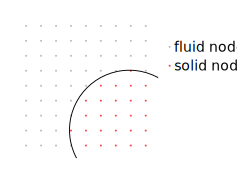
\includegraphics[width=\singleimagewidth]{chapters/figures/lbm/dem-to-lbm-mapping.pdf}
	\caption{An example of the mapping process from DEM to LBM structures. Nodes are assigned as fluid or solid based on relative location of pebble centroid and radius. Here we have a resolution of 9 (\textit{i.e.} 9 nodes per pebble diameter).}\label{fig:dem-2-lbm-example1}
\end{figure}
\begin{figure}[ht]
	\centering
	\includegraphics[width=\doubleimagewidth]{chapters/figures/lbm/lbm-pebble-res25.png}
	\caption{A three-dimensional DEM pebble as imported into the LBM lattice with a resolution of 25.}\label{fig:dem-2-lbm-example2}
\end{figure}
\begin{figure}[ht]
	\centering
	\includegraphics[width=\doubleimagewidth]{chapters/figures/lbm/crossSection0024.jpg}
	\caption{A two-dimensional slice of a DEM pebble bed as imported into the LBM lattice with a resolution of 25.}\label{fig:dem-2-lbm-example3}
\end{figure}
\begin{figure}[ht]
	\centering
	\includegraphics[width=\textwidth]{chapters/figures/lbm/palabos_packing_fraction}
	\caption{The digital packing fraction was measured at all slices through the height of the pebble bed. When the average value equaled the expected value, the mapping from DEM to LBM was considered consistent.}\label{fig:dem-2-lbm-packing-fraction}
\end{figure}

In the example of Fig.~\ref{fig:dem-2-lbm-example1}, the resolution is only 9. Thus 9 nodes are needed to span the diameter of a single pebble and the lattice spacing is $\delta_x = 1/9$. In the second example shown in Fig.~\ref{fig:dem-2-lbm-example2}, we see a pebble in three dimensions that has been mapped onto the LBM nodes with a resolution of 25 (thus $\delta_x = 1/25$). The trade-off between a small lattice spacing is in the ability to resolve the spherical surface of the pebble, stability, and even the ability to resolve a proper packing fraction in the pebble bed. 

Shown in Fig.~\ref{fig:dem-2-lbm-example3} is a single slice of a pebble bed with a resolution of 25 as it is mapped into LBM. Here, black pixels represent solid and white pixels are fluid. Because we are representing the surfaces of curved objects with straight lines, at the point of contact between pebbles, the mapping from DEM to LBM would occasionally over-predict the overlap between pebbles. This was measured numerically by comparing the number of white pixels to black pixels in each slice -- the digital equivalent of a packing fraction,
\begin{equation}
	\phi_{d,j} = \frac{N_\text{black}}{N_\text{white}}
\end{equation}

The total digital packing fraction of the ensemble, as mapped into LBM, is simply
\begin{equation}
	\phi_d = \frac{1}{J}\sum_j^J\phi_{d,j}
\end{equation}

where there are $J$ total slices. For example, we see in Fig.~\ref{fig:dem-2-lbm-packing-fraction} a plot of the digital packing fraction moving through the pebble bed. The digital mapping of DEM onto LBM was tweaked with a radius magnification parameter until the digital packing fraction matched the calculated packing fraction from DEM. When the error between digital and continuous packing fractions was small, as calculated by
\begin{equation}
	\Phi_{err} = \frac{|\phi_d - \phi|}{\phi} < 10^{-4}
\end{equation}
I considered the mapping from DEM to LBM to be consistent.
\FloatBarrier
\subsection{Numerical Implementation of LBM}\label{sec:lbm-solver}

As usual, the packing structure of our pebble bed is rendered with the code LIGGGHTS. Details of the software are described in \cref{sec:dem-solver}. The DEM solver is a highly parallel C++ code based on the Molecular Dynamics (MD) code LAMMPS.\cite{Plimpton1995} 

The translation between the DEM packing and LBM nodal network is done with in-house Python scripts to discretize and digitize the `spherical' information of DEM into LBM.

To solve the lattice-Boltzmann collision and streaming equations, we make use of the open-source code maintained by FlowKit Ltd named Palabos.\cite{Flow} The Palabos library provides an interface for quick implementation of lattice-Boltzmann models in C++. Implemented models include the BGK and thermal flows with the Boussinesq approximation, among many others. They are all run on the possible grids of D2Q9, D3Q13, D3Q15, D3Q19, or D3Q27. Zou/He, periodic, and bounce-back conditions are built into the LB kernel; implementation of Dirichlet or Neumann conditions with velocity or pressure are also possible. The software is freely available under the terms of the open-source AGPLv3 license.\cite{FreeSoftwareFoundationInc.2007} All mentioned models and ingredients are parallelized with MPI, including the I/O operations that are implemented in terms of MPI’s Parallel I/O API.

\section{Summary of LBM Modeling Development}

While concurrently developing the dynamic-coupling tools for the CFD-DEM models, I recognized the potential need for modeling the meandering path of low-$\Re$ flow of helium in our packed bed with heat generation. The sacrifice we make to achieve the numerical fidelity is that in this implementation of fluid-particle interaction we have a static coupling. The pebble-scale micromechanical interaction information for pebble damage modeling is still solved transiently in the DEM computations. When the bed is settled, a snapshot of the structure is discretized and loaded into the LBM solver which then calculates temperature and velocity fields of both solid and fluid phases. There is no cross-communication in this technique as the packing structure is effectively frozen during the LBM calculations.

The LBM approach was chosen in place of finite element or finite volume methodology because of issues with discretization of meshes in a three dimensional packed bed with interstitial gas. There are techniques to handle packed beds with continuum fluid mechanics software, but the size of packed beds we are interested in make the FEM approach intractable.

Furthermore, the simple LBM formulation of enforcing no-slip conditions on complex geometry is trivially realized with bounce-back rules on distribution functions. The multi-relaxation-time lattices for momentum and energy offer complete modeling of complex geometry and conjugate heat transfer with far less computational overhead compared to FEM models.